
%% bare_conf.tex
%% V1.3
%% 2007/01/11
%% by Michael Shell
%% See:
%% http://www.michaelshell.org/
%% for current contact information.
%%
%% This is a skeleton file demonstrating the use of IEEEtran.cls
%% (requires IEEEtran.cls version 1.7 or later) with an IEEE conference paper.
%%
%% Support sites:
%% http://www.michaelshell.org/tex/ieeetran/
%% http://www.ctan.org/tex-archive/macros/latex/contrib/IEEEtran/
%% and
%% http://www.ieee.org/

%%*************************************************************************
%% Legal Notice:
%% This code is offered as-is without any warranty either expressed or
%% implied; without even the implied warranty of MERCHANTABILITY or
%% FITNESS FOR A PARTICULAR PURPOSE! 
%% User assumes all risk.
%% In no event shall IEEE or any contributor to this code be liable for
%% any damages or losses, including, but not limited to, incidental,
%% consequential, or any other damages, resulting from the use or misuse
%% of any information contained here.
%%
%% All comments are the opinions of their respective authors and are not
%% necessarily endorsed by the IEEE.
%%
%% This work is distributed under the LaTeX Project Public License (LPPL)
%% ( http://www.latex-project.org/ ) version 1.3, and may be freely used,
%% distributed and modified. A copy of the LPPL, version 1.3, is included
%% in the base LaTeX documentation of all distributions of LaTeX released
%% 2003/12/01 or later.
%% Retain all contribution notices and credits.
%% ** Modified files should be clearly indicated as such, including  **
%% ** renaming them and changing author support contact information. **
%%
%% File list of work: IEEEtran.cls, IEEEtran_HOWTO.pdf, bare_adv.tex,
%%                    bare_conf.tex, bare_jrnl.tex, bare_jrnl_compsoc.tex
%%*************************************************************************

% *** Authors should verify (and, if needed, correct) their LaTeX system  ***
% *** with the testflow diagnostic prior to trusting their LaTeX platform ***
% *** with production work. IEEE's font choices can trigger bugs that do  ***
% *** not appear when using other class files.                            ***
% The testflow support page is at:
% http://www.michaelshell.org/tex/testflow/



% Note that the a4paper option is mainly intended so that authors in
% countries using A4 can easily print to A4 and see how their papers will
% look in print - the typesetting of the document will not typically be
% affected with changes in paper size (but the bottom and side margins will).
% Use the testflow package mentioned above to verify correct handling of
% both paper sizes by the user's LaTeX system.
%
% Also note that the "draftcls" or "draftclsnofoot", not "draft", option
% should be used if it is desired that the figures are to be displayed in
% draft mode.
%
\documentclass[conference]{./style/IEEEtran}
% Add the compsoc option for Computer Society conferences.
%
% If IEEEtran.cls has not been installed into the LaTeX system files,
% manually specify the path to it like:
% \documentclass[conference]{../sty/IEEEtran}





% Some very useful LaTeX packages include:
% (uncomment the ones you want to load)


% *** MISC UTILITY PACKAGES ***
%
%\usepackage{ifpdf}
% Heiko Oberdiek's ifpdf.sty is very useful if you need conditional
% compilation based on whether the output is pdf or dvi.
% usage:
% \ifpdf
%   % pdf code
% \else
%   % dvi code
% \fi
% The latest version of ifpdf.sty can be obtained from:
% http://www.ctan.org/tex-archive/macros/latex/contrib/oberdiek/
% Also, note that IEEEtran.cls V1.7 and later provides a builtin
% \ifCLASSINFOpdf conditional that works the same way.
% When switching from latex to pdflatex and vice-versa, the compiler may
% have to be run twice to clear warning/error messages.






% *** CITATION PACKAGES ***
%
%\usepackage{cite}
% cite.sty was written by Donald Arseneau
% V1.6 and later of IEEEtran pre-defines the format of the cite.sty package
% \cite{} output to follow that of IEEE. Loading the cite package will
% result in citation numbers being automatically sorted and properly
% "compressed/ranged". e.g., [1], [9], [2], [7], [5], [6] without using
% cite.sty will become [1], [2], [5]--[7], [9] using cite.sty. cite.sty's
% \cite will automatically add leading space, if needed. Use cite.sty's
% noadjust option (cite.sty V3.8 and later) if you want to turn this off.
% cite.sty is already installed on most LaTeX systems. Be sure and use
% version 4.0 (2003-05-27) and later if using hyperref.sty. cite.sty does
% not currently provide for hyperlinked citations.
% The latest version can be obtained at:
% http://www.ctan.org/tex-archive/macros/latex/contrib/cite/
% The documentation is contained in the cite.sty file itself.






% *** GRAPHICS RELATED PACKAGES ***
%
\ifCLASSINFOpdf
  % \usepackage[pdftex]{graphicx}
  % declare the path(s) where your graphic files are
  % \graphicspath{{../pdf/}{../jpeg/}}
  % and their extensions so you won't have to specify these with
  % every instance of \includegraphics
  % \DeclareGraphicsExtensions{.pdf,.jpeg,.png}
\else
  % or other class option (dvipsone, dvipdf, if not using dvips). graphicx
  % will default to the driver specified in the system graphics.cfg if no
  % driver is specified.
  % \usepackage[dvips]{graphicx}
  % declare the path(s) where your graphic files are
  % \graphicspath{{../eps/}}
  % and their extensions so you won't have to specify these with
  % every instance of \includegraphics
  % \DeclareGraphicsExtensions{.eps}
\fi
% graphicx was written by David Carlisle and Sebastian Rahtz. It is
% required if you want graphics, photos, etc. graphicx.sty is already
% installed on most LaTeX systems. The latest version and documentation can
% be obtained at: 
% http://www.ctan.org/tex-archive/macros/latex/required/graphics/
% Another good source of documentation is "Using Imported Graphics in
% LaTeX2e" by Keith Reckdahl which can be found as epslatex.ps or
% epslatex.pdf at: http://www.ctan.org/tex-archive/info/
%
% latex, and pdflatex in dvi mode, support graphics in encapsulated
% postscript (.eps) format. pdflatex in pdf mode supports graphics
% in .pdf, .jpeg, .png and .mps (metapost) formats. Users should ensure
% that all non-photo figures use a vector format (.eps, .pdf, .mps) and
% not a bitmapped formats (.jpeg, .png). IEEE frowns on bitmapped formats
% which can result in "jaggedy"/blurry rendering of lines and letters as
% well as large increases in file sizes.
%
% You can find documentation about the pdfTeX application at:
% http://www.tug.org/applications/pdftex





% *** MATH PACKAGES ***
%
%\usepackage[cmex10]{amsmath}
% A popular package from the American Mathematical Society that provides
% many useful and powerful commands for dealing with mathematics. If using
% it, be sure to load this package with the cmex10 option to ensure that
% only type 1 fonts will utilized at all point sizes. Without this option,
% it is possible that some math symbols, particularly those within
% footnotes, will be rendered in bitmap form which will result in a
% document that can not be IEEE Xplore compliant!
%
% Also, note that the amsmath package sets \interdisplaylinepenalty to 10000
% thus preventing page breaks from occurring within multiline equations. Use:
%\interdisplaylinepenalty=2500
% after loading amsmath to restore such page breaks as IEEEtran.cls normally
% does. amsmath.sty is already installed on most LaTeX systems. The latest
% version and documentation can be obtained at:
% http://www.ctan.org/tex-archive/macros/latex/required/amslatex/math/





% *** SPECIALIZED LIST PACKAGES ***
%
%\usepackage{algorithmic}
% algorithmic.sty was written by Peter Williams and Rogerio Brito.
% This package provides an algorithmic environment fo describing algorithms.
% You can use the algorithmic environment in-text or within a figure
% environment to provide for a floating algorithm. Do NOT use the algorithm
% floating environment provided by algorithm.sty (by the same authors) or
% algorithm2e.sty (by Christophe Fiorio) as IEEE does not use dedicated
% algorithm float types and packages that provide these will not provide
% correct IEEE style captions. The latest version and documentation of
% algorithmic.sty can be obtained at:
% http://www.ctan.org/tex-archive/macros/latex/contrib/algorithms/
% There is also a support site at:
% http://algorithms.berlios.de/index.html
% Also of interest may be the (relatively newer and more customizable)
% algorithmicx.sty package by Szasz Janos:
% http://www.ctan.org/tex-archive/macros/latex/contrib/algorithmicx/




% *** ALIGNMENT PACKAGES ***
%
%\usepackage{array}
% Frank Mittelbach's and David Carlisle's array.sty patches and improves
% the standard LaTeX2e array and tabular environments to provide better
% appearance and additional user controls. As the default LaTeX2e table
% generation code is lacking to the point of almost being broken with
% respect to the quality of the end results, all users are strongly
% advised to use an enhanced (at the very least that provided by array.sty)
% set of table tools. array.sty is already installed on most systems. The
% latest version and documentation can be obtained at:
% http://www.ctan.org/tex-archive/macros/latex/required/tools/


%\usepackage{mdwmath}
%\usepackage{mdwtab}
% Also highly recommended is Mark Wooding's extremely powerful MDW tools,
% especially mdwmath.sty and mdwtab.sty which are used to format equations
% and tables, respectively. The MDWtools set is already installed on most
% LaTeX systems. The lastest version and documentation is available at:
% http://www.ctan.org/tex-archive/macros/latex/contrib/mdwtools/


% IEEEtran contains the IEEEeqnarray family of commands that can be used to
% generate multiline equations as well as matrices, tables, etc., of high
% quality.


%\usepackage{eqparbox}
% Also of notable interest is Scott Pakin's eqparbox package for creating
% (automatically sized) equal width boxes - aka "natural width parboxes".
% Available at:
% http://www.ctan.org/tex-archive/macros/latex/contrib/eqparbox/





% *** SUBFIGURE PACKAGES ***
%\usepackage[tight,footnotesize]{subfigure}
% subfigure.sty was written by Steven Douglas Cochran. This package makes it
% easy to put subfigures in your figures. e.g., "Figure 1a and 1b". For IEEE
% work, it is a good idea to load it with the tight package option to reduce
% the amount of white space around the subfigures. subfigure.sty is already
% installed on most LaTeX systems. The latest version and documentation can
% be obtained at:
% http://www.ctan.org/tex-archive/obsolete/macros/latex/contrib/subfigure/
% subfigure.sty has been superceeded by subfig.sty.



%\usepackage[caption=false]{caption}
%\usepackage[font=footnotesize]{subfig}
% subfig.sty, also written by Steven Douglas Cochran, is the modern
% replacement for subfigure.sty. However, subfig.sty requires and
% automatically loads Axel Sommerfeldt's caption.sty which will override
% IEEEtran.cls handling of captions and this will result in nonIEEE style
% figure/table captions. To prevent this problem, be sure and preload
% caption.sty with its "caption=false" package option. This is will preserve
% IEEEtran.cls handing of captions. Version 1.3 (2005/06/28) and later 
% (recommended due to many improvements over 1.2) of subfig.sty supports
% the caption=false option directly:
%\usepackage[caption=false,font=footnotesize]{subfig}
%
% The latest version and documentation can be obtained at:
% http://www.ctan.org/tex-archive/macros/latex/contrib/subfig/
% The latest version and documentation of caption.sty can be obtained at:
% http://www.ctan.org/tex-archive/macros/latex/contrib/caption/




% *** FLOAT PACKAGES ***
%
%\usepackage{fixltx2e}
% fixltx2e, the successor to the earlier fix2col.sty, was written by
% Frank Mittelbach and David Carlisle. This package corrects a few problems
% in the LaTeX2e kernel, the most notable of which is that in current
% LaTeX2e releases, the ordering of single and double column floats is not
% guaranteed to be preserved. Thus, an unpatched LaTeX2e can allow a
% single column figure to be placed prior to an earlier double column
% figure. The latest version and documentation can be found at:
% http://www.ctan.org/tex-archive/macros/latex/base/



%\usepackage{stfloats}
% stfloats.sty was written by Sigitas Tolusis. This package gives LaTeX2e
% the ability to do double column floats at the bottom of the page as well
% as the top. (e.g., "\begin{figure*}[!b]" is not normally possible in
% LaTeX2e). It also provides a command:
%\fnbelowfloat
% to enable the placement of footnotes below bottom floats (the standard
% LaTeX2e kernel puts them above bottom floats). This is an invasive package
% which rewrites many portions of the LaTeX2e float routines. It may not work
% with other packages that modify the LaTeX2e float routines. The latest
% version and documentation can be obtained at:
% http://www.ctan.org/tex-archive/macros/latex/contrib/sttools/
% Documentation is contained in the stfloats.sty comments as well as in the
% presfull.pdf file. Do not use the stfloats baselinefloat ability as IEEE
% does not allow \baselineskip to stretch. Authors submitting work to the
% IEEE should note that IEEE rarely uses double column equations and
% that authors should try to avoid such use. Do not be tempted to use the
% cuted.sty or midfloat.sty packages (also by Sigitas Tolusis) as IEEE does
% not format its papers in such ways.





% *** PDF, URL AND HYPERLINK PACKAGES ***
%
%\usepackage{url}
% url.sty was written by Donald Arseneau. It provides better support for
% handling and breaking URLs. url.sty is already installed on most LaTeX
% systems. The latest version can be obtained at:
% http://www.ctan.org/tex-archive/macros/latex/contrib/misc/
% Read the url.sty source comments for usage information. Basically,
% \url{my_url_here}.





% *** Do not adjust lengths that control margins, column widths, etc. ***
% *** Do not use packages that alter fonts (such as pslatex).         ***
% There should be no need to do such things with IEEEtran.cls V1.6 and later.
% (Unless specifically asked to do so by the journal or conference you plan
% to submit to, of course. )


\usepackage[usenames]{color}
\usepackage[latin1]{inputenc}
\usepackage{amsmath}
\usepackage{amsfonts}
\usepackage{amssymb}
\usepackage{epsfig}

\def\eg{{\it e.g., \/}}
\def\ie{{\it i.e., \/}}
\def\etal{{\it et al.\/}}
\def\viz{{\it viz.,\/ }}

% correct bad hyphenation here
\hyphenation{op-tical net-works semi-conduc-tor}


\begin{document}
%
% paper title
% can use linebreaks \\ within to get better formatting as desired
%\title{Bare Demo of IEEEtran.cls for Conferences}

\title{Heavyweight Pattern Mining in Attributed Flow Graphs} 

% author names and affiliations
% use a multiple column layout for up to three different
% affiliations
%\author{\IEEEauthorblockN{Michael Shell}
%\IEEEauthorblockA{School of Electrical and\\Computer Engineering\\
%Georgia Institute of Technology\\
%Atlanta, Georgia 30332--0250\\
%Email: http://www.michaelshell.org/contact.html}
%\and
%\IEEEauthorblockN{Homer Simpson}
%\IEEEauthorblockA{Twentieth Century Fox\\
%Springfield, USA\\
%Email: homer@thesimpsons.com}
%\and
%\IEEEauthorblockN{James Kirk\\ and Montgomery Scott}
%\IEEEauthorblockA{Starfleet Academy\\
%San Francisco, California 96678-2391\\
%Telephone: (800) 555--1212\\
%Fax: (888) 555--1212}}

% conference papers do not typically use \thanks and this command
% is locked out in conference mode. If really needed, such as for
% the acknowledgment of grants, issue a \IEEEoverridecommandlockouts
% after \documentclass

% for over three affiliations, or if they all won't fit within the width
% of the page, use this alternative format:
% 
%\author{\IEEEauthorblockN{Michael Shell\IEEEauthorrefmark{1},
%Homer Simpson\IEEEauthorrefmark{2},
%James Kirk\IEEEauthorrefmark{3}, 
%Montgomery Scott\IEEEauthorrefmark{3} and
%Eldon Tyrell\IEEEauthorrefmark{4}}
%\IEEEauthorblockA{\IEEEauthorrefmark{1}School of Electrical and Computer Engineering\\
%Georgia Institute of Technology,
%Atlanta, Georgia 30332--0250\\ Email: see http://www.michaelshell.org/contact.html}
%\IEEEauthorblockA{\IEEEauthorrefmark{2}Twentieth Century Fox, Springfield, USA\\
%Email: homer@thesimpsons.com}
%\IEEEauthorblockA{\IEEEauthorrefmark{3}Starfleet Academy, San Francisco, California 96678-2391\\
%Telephone: (800) 555--1212, Fax: (888) 555--1212}
%\IEEEauthorblockA{\IEEEauthorrefmark{4}Tyrell Inc., 123 Replicant Street, Los Angeles, California %90210--4321}}

\author{\IEEEauthorblockN{Carolina Sim\~oes Gomes}
\IEEEauthorblockA{Intuit Canada\\
Edmonton, AB, Canada\\ Email: carolina.sgomes@gmail.com}
\\
\\
\IEEEauthorblockN{Joran Siu}
\IEEEauthorblockA{IBM Canada Software Laboratory\\
Markham, ON, Canada\\
Email: joransiu@ibm.ca}
\and
\IEEEauthorblockN{Jos\'e Nelson Amaral}
\IEEEauthorblockA{Department of Computing Science\\
University of Alberta\\
Edmonton, AB, Canada\\
Email: amaral@cs.ualberta.ca}
\\
\IEEEauthorblockN{Li Ding}
\IEEEauthorblockA{Amazon Canada\\
Toronto, ON, Canada\\
Email: ldingca@yahoo.com}
\and
\IEEEauthorblockN{Joerg Sander}
\IEEEauthorblockA{Department of Computing Science\\
University of Alberta\\
Edmonton, AB, Canada\\
Email: jsander@ualberta.ca}}






% use for special paper notices
%\IEEEspecialpapernotice{(Invited Paper)}

% make the title area
\maketitle

\begin{abstract}
%\boldmath
This paper defines a new problem - heavyweight pattern mining in attributed flow graphs. The problem can be described as the discovery of patterns in flow graphs that have sets of attributes associated with their nodes. A connection between nodes is represented as a directed edge. The amount of load that goes through a path between nodes, or the frequency of transmission of such load between nodes, is represented as edge weights. A heavyweight pattern is a sub-set of attributes, found in a dataset of attributed flow graphs, that are connected by edges and have a computed weight higher than an user-defined threshold. A new algorithm called AFGMiner is introduced, the first one to our knowledge that finds heavyweight patterns in a dataset of attributed flow graphs and associates each pattern with its occurrences. The paper also describes a new tool for compiler engineers, HEPMiner, that applies the AFGMiner algorithm to Profile-based Program Analysis modeled as a heavyweight pattern mining problem.
\end{abstract}

% IEEEtran.cls defaults to using nonbold math in the Abstract.
% This preserves the distinction between vectors and scalars. However,
% if the conference you are submitting to favors bold math in the abstract,
% then you can use LaTeX's standard command \boldmath at the very start
% of the abstract to achieve this. Many IEEE journals/conferences frown on
% math in the abstract anyway.

% no keywords




% For peer review papers, you can put extra information on the cover
% page as needed:
% \ifCLASSOPTIONpeerreview
% \begin{center} \bfseries EDICS Category: 3-BBND \end{center}
% \fi
%
% For peerreview papers, this IEEEtran command inserts a page break and
% creates the second title. It will be ignored for other modes.
\IEEEpeerreviewmaketitle

\section{Introduction}
	\label{sec:intro}
	Flow graphs are an abstraction used to represent elements (\eg digital data, goods, electric current) that travel through a network of nodes (\eg computers, physical locations, circuit parts). Flow graphs are often used in the modelling of logistics problems. An attributed flow graph (AFG) is a single-entry/single-exit graph with a \emph{source node} that has no incoming edges and a \emph{sink node} with no outgoing edges.The flow starts in the source node and is directed to the sink node. All other nodes in the AFG, if they exist, must have at least one incoming and one outgoing edge. In addition, AFGs have attributes in their nodes, representing e.g. typec of goods at a given network node, and weights in nodes and edges, representing e.g. the amount of goods stores at that node and flowing between any two nodes. An example of an AFG is shown in Figure~\ref{fig:AFG}.

\begin{figure}[htp]
\centering
\begin{tabular}{cc}
 %   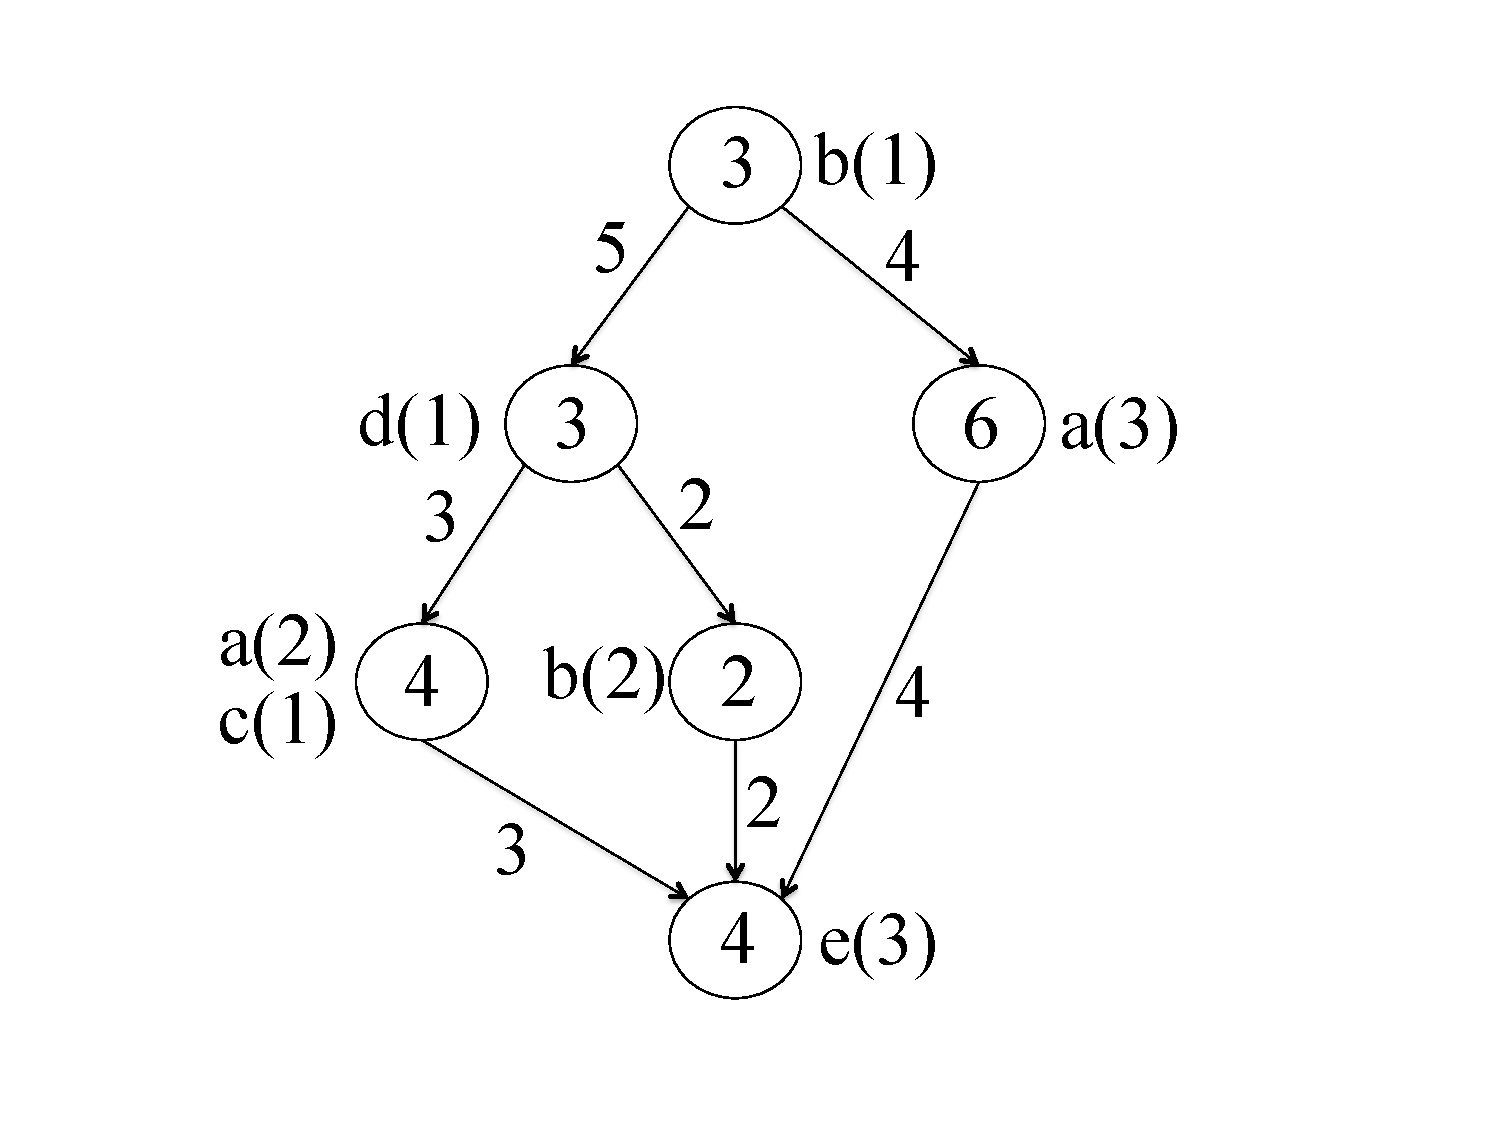
\includegraphics[scale=0.2]{figures/attributed_flow_graph2.eps}
  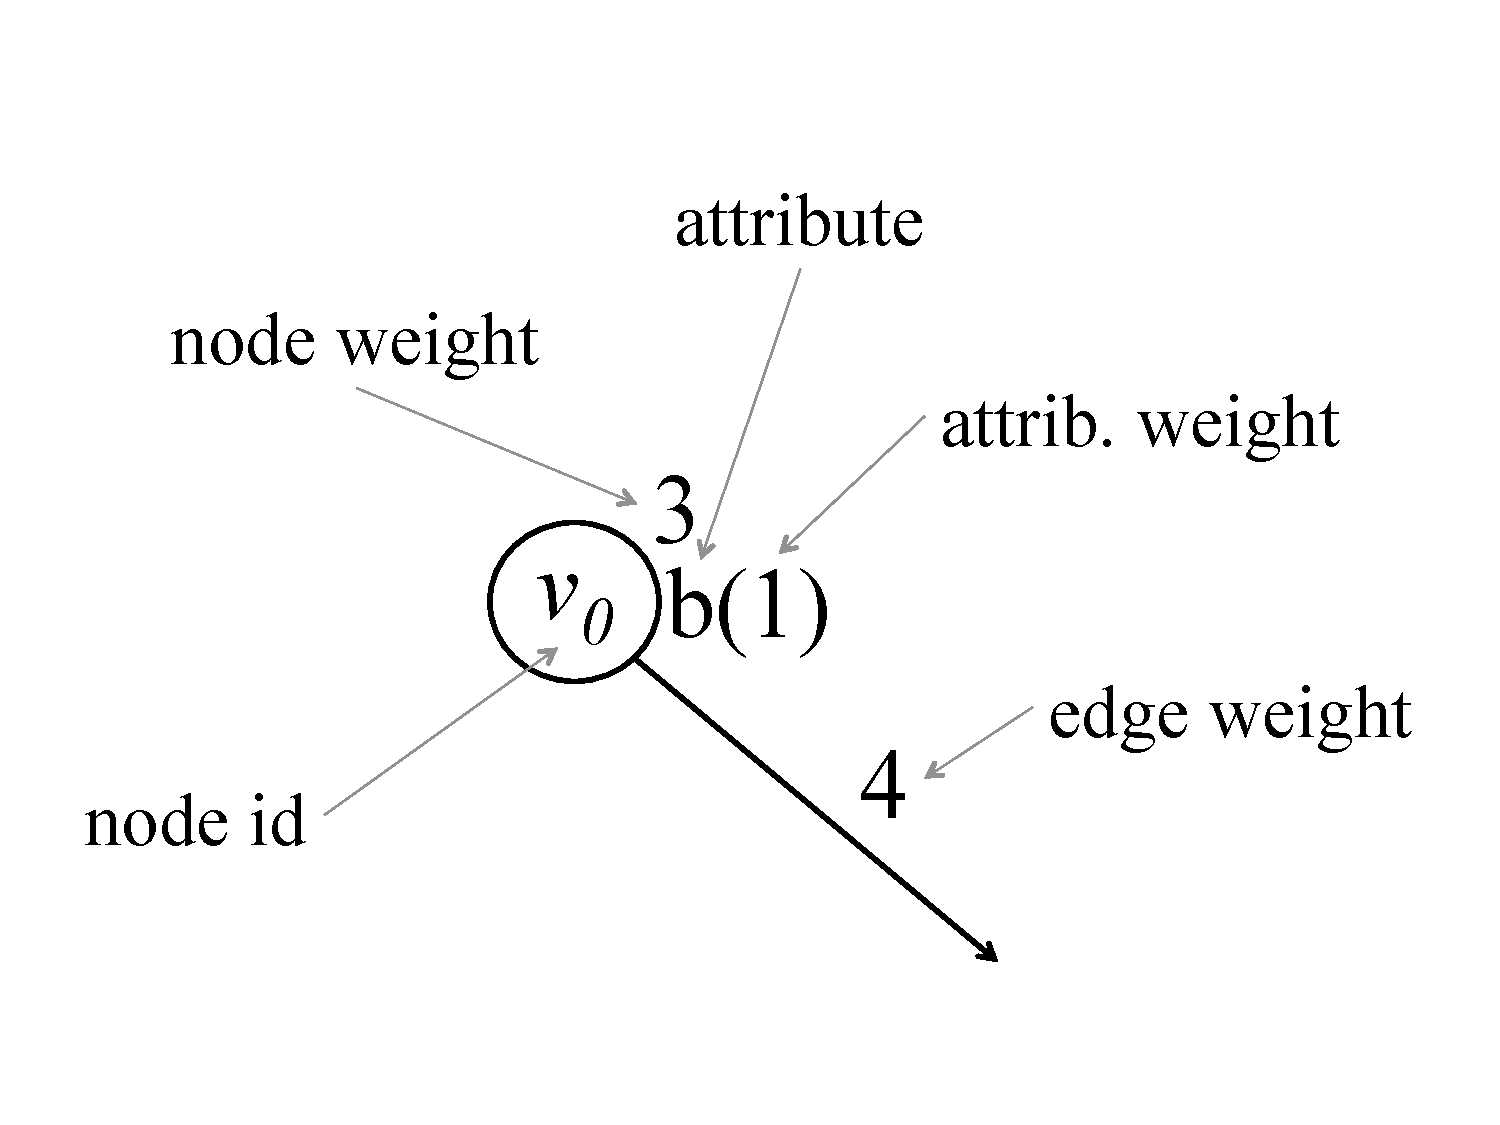
\includegraphics[scale=0.15]{figures/attributed_flow_graph_descpr.pdf} &
  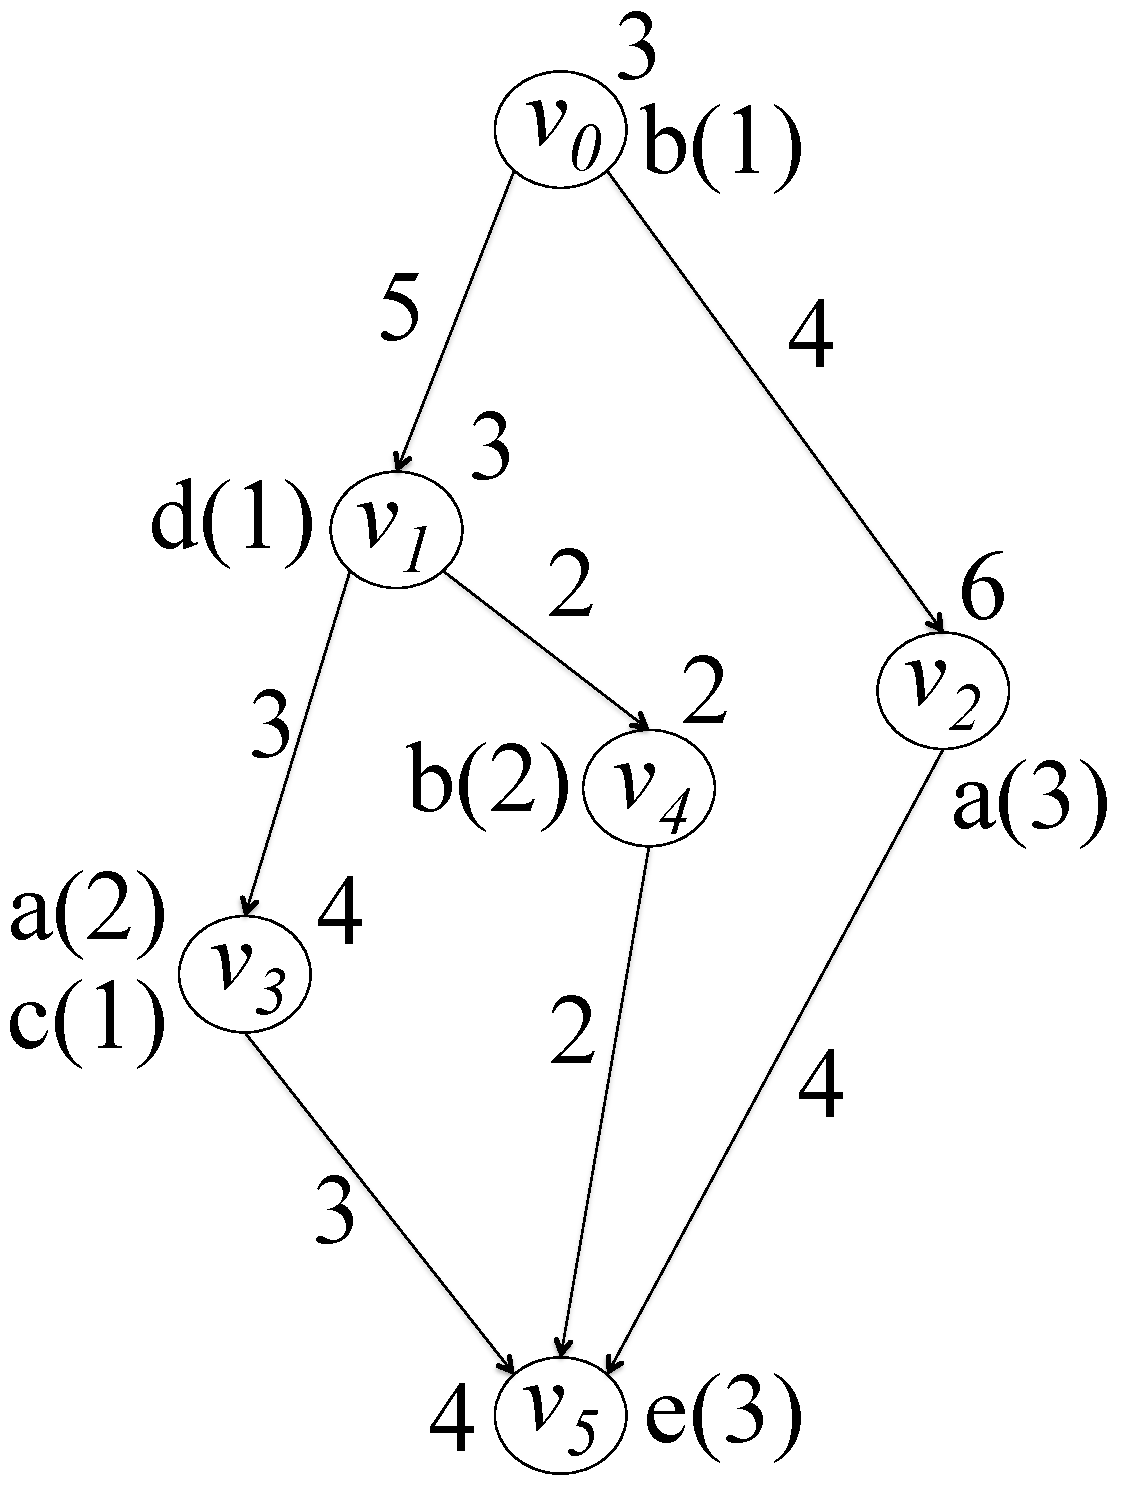
\includegraphics[scale=0.15]{figures/attributed_flow_graph3.pdf}\\
  (a) Elements of an AFG & (b) Example
\end{tabular}
    \caption{Example of attributed flow graph.}
    \label{fig:AFG}  
\end{figure}

Existing graph-mining algorithms are all severely limited in their applicability to AFGs. None of them is able to find general sub-graph patterns in AFGs that take into account multiple node attributes as well as weights in nodes and edges. The only work on mining patterns in AFGs is the FlowGSP algorithm proposed by \emph{Jocksch~\etal}~\cite{FlowGSP}. However, FlowGSP can only find sub-path patterns, while the algorithm described in this work finds all the patterns that FlowGSP does and additional patterns that encompass multiple sub-paths in the dataset.  

This paper presents AFGMiner, the first algorithm, to the best of our knowledge, to address the problem of mining AFGs for general sub-graph patterns. AFGMiner takes as input a set of AFGs and a support measure $MinSup$ that may be formulated by taking into account the attribute weights, node weights and edge weights of the occurrences of patterns. AFGMiner returns all patterns $P$, called \emph{heavyweight patterns}, whose support $MinSup(P)$ is higher than a threshold. This threshold is user-specified as commonly assumed in pattern-mining approaches.
The main contributions of this paper are as follows: 

\begin{enumerate}
\item Definition of the Attributed-Flow-Graph Mining problem to find Heavyweight Patterns.

\item Development of different versions of AFGMiner, an algorithm that mines for heavyweight patterns in attributed flow graphs, including a parallel version with a work-distribution heuristic to maintain workload balance between multiple threads.

\item Development of HEPMiner, a tool that automates the analysis of hardware-instrumented profiles, as an application of AFGMiner. Patterns discovered by HEPMiner indicate potential, non-obvious, opportunities for compiler and architecture-design improvements.

\item Complexity and performance analysis of AFGMiner, comparison against the FlowGSP algorithm and qualitative analysis of patterns found by HEPMiner when applied to the DayTrader benchmark running on IBM's WebSphere Application Server~\cite{WAS}.
\end{enumerate} 






\section{Problem Definition}
        \label{sec:ProblemDef}
        \def\eg{{\it e.g., \/}}
\def\ie{{\it i.e., \/}}
\def\etal{{\it et al.\/}}
\def\viz{{\it viz.,\/ }}

An attributed flow graph (AFG) $G$, that belongs to a dataset $DS$ of AFGs, is defined as $G = \langle V, E, A, \alpha, w^E, w^V, w^{A,V}, l \rangle$ where:

\begin{enumerate}
\item $V$ is a set of nodes.

\item $E$ is a set of directed edges $(v_a, v_b)$ where $v_a, v_b \in V$.

\item $A$ is the set of all possible attributes.

\item $\alpha$ is a function mapping nodes $v \in V$ to a subset of attributes, \ie $\alpha(v) = \{a_1, ..., a_k\}$,  $a_i \in A$, $1 \leq i \leq k$.

\item $w^E$ is a function assigning a weight $w \in [0,1]$ to each edge $e \in E$ so that $\Sigma_{e \in E_{DS}}w^E(e)$ $ = 1$ where $E_{DS}$ is the set of edges from all AFGs that belong to $DS$, \ie $w^E$ is normalized over $DS$.  

\item $w^V$ is a function assigning a weight $w \in [0,1]$ to each node $v \in V$ so that $\Sigma_{v \in V_{DS}}w^V(v)$ $ = 1$ where $V_{DS}$ is the set of nodes from all AFGs that belong to $DS$, \ie $w^V$ is normalized over $DS$.

\item $w^{A,V}$ is a function assigning a weight $w \in [0,1]$ to each attribute $a$ of each node $v \in V$, $a \in \alpha(v)$, with the constraint that $w^{A,V}(a) \leq w^V(v)$.

\item $l$ is a function assigning a unique integer label $l(v)$ to each node $v \in V$, according to a depth-first traversal of the graph. $l(V)$ denotes the result of applying the labeling function to all nodes in $V$. Given an edge $(v_i, v_j)$, the edge is called a \emph{forward} edge if $l(v_i) < l(v_j)$; otherwise, if $l(v_i) \geq l(v_j)$ the edge is called a \emph{backward} edge or \emph{back-edge}; the node $v_i$ is called the edge's \emph{from-node} and the node $v_j$ is called the edge's \emph{to-node}.   

\item $G$ is a flow graph, \ie for any node $v^*$ it holds that
$\Sigma_{(x, v^*) \in E}w^E((x, v^*))$ $= \Sigma_{(v^*, y) \in E}w^E((v^*, y))$.

\end{enumerate}

A directed graph $g = \langle V_g, E_g, A_g, \alpha_g, w_g^E, w_g^V, w_g^{A,V}, l_g \rangle$ is a \emph{sub-graph} of $G$, if $V_g$ is a subset of the nodes in $G$, $E_g$ is a subset of the edges in $G$ that exist between nodes in $V_g$, A is a subset of the attributes in $G$, and the functions $\alpha_g, w_g^E, w_g^V, w_g^{A,V}, l_g$ are the corresponding functions in $G$, restricted to the corresponding domains of nodes, edges and attributes in $g$. 

A \emph{pattern} is a graph $P = <V_P, E_P, A, \alpha>$, where $V_P$ is a set of nodes with attributes from $A$ associated to them by $\alpha$, and $E_P$ is a set of directed edges; note that a pattern does not include weights.  A pattern is an abstraction in which the nodes represent sets of attributes that are relevant under a \emph{support criteria}, and the edges represent an ordering for such attribute sets.

An \emph{occurrence} $g$ of a pattern $P$ is a sub-graph of $G$ that ``matches $P$ with a maximum gap size $k_{max}$''; $g$ \emph{matches} $P$ \emph{with a maximum gap size} $k_{max}$ if there is a function $m$ that maps every node $v$ in $P$ to a node in $g$ so that for every edge $(v_i, v_j)$ in $P$, there is a path in $g$ that starts at node $m(v_i)$ and ends at node $m(v_j)$, and that has at most $k_{max}$ nodes between $m(v_i)$ and $m(v_j)$. This definition of an occurrence of a pattern allows a number $k_{max}$ of ``mismatches'' or ``don't-care nodes'' when mapping each node in the pattern $P$ to a sub-graph in G, and $k_{max}$ can be chosen by a user in order to allow approximate matches in applications where such an approach is useful. A $k_{max}$-match of a pattern $P$ is an occurrence $g_P$ of $P$ that was found by using a maximum gap size of $k_{max}$. As an example, in Figure~\ref{fig:GapExample} we have a pattern on the left and an AFG in which a 0-match, an 1-match and a 2-match of the pattern can be found. 

\begin{figure}[h!]
\centering
%    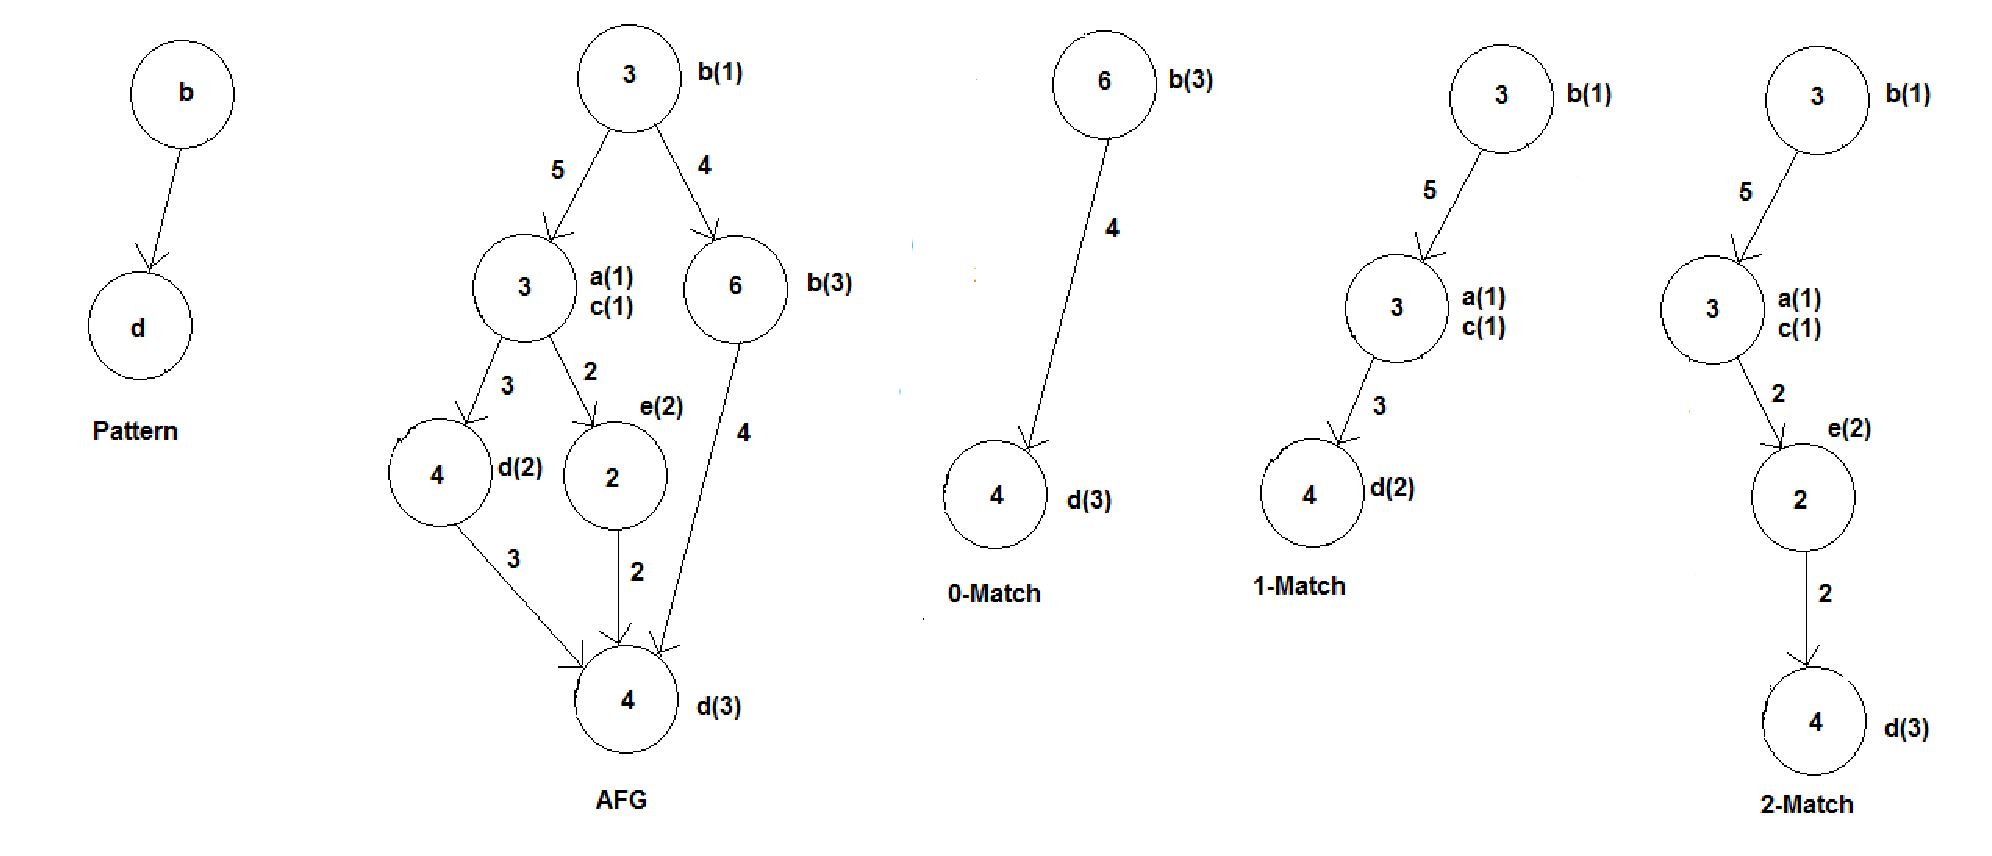
\includegraphics[scale=0.2]{figures/match_example.eps}
      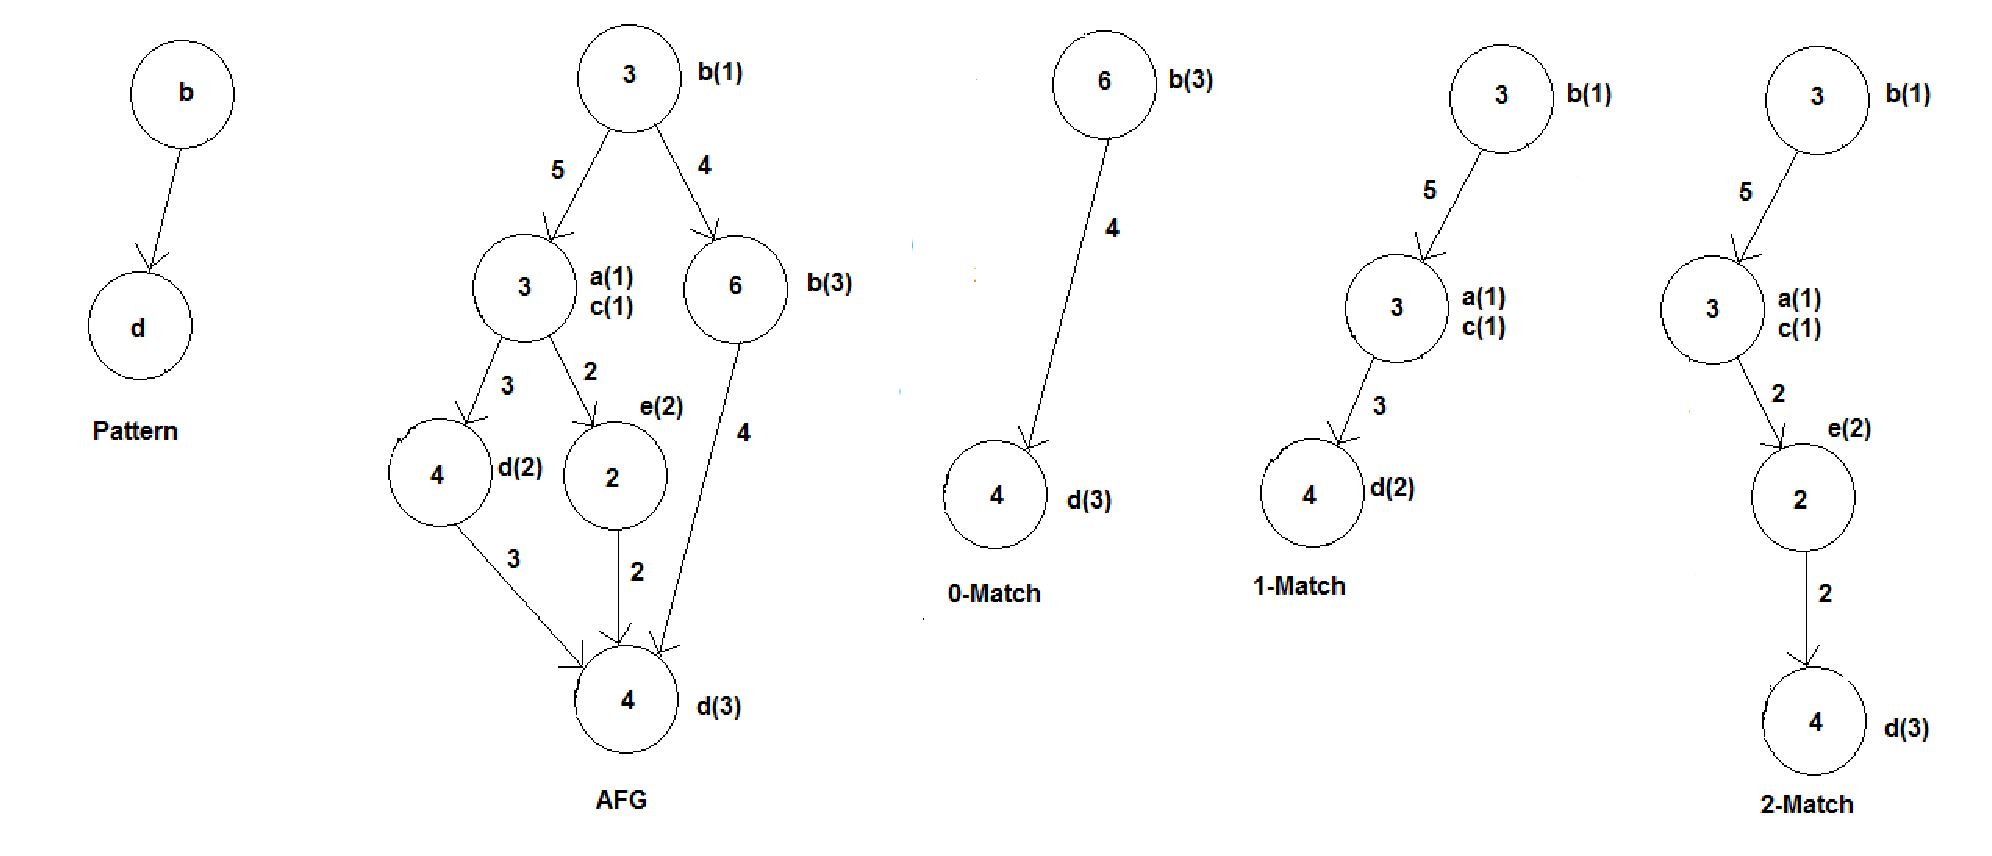
\includegraphics[scale=0.25]{figures/match_example.pdf}
    \caption{Example of k-matches of a pattern.}
    \label{fig:GapExample}  
\end{figure}

Assume a dataset $DS$ of AFGs, a \emph{support measure} $MinSup$ that defines the minimum support of patterns $P$ in $DS$, the maximum number of attributes allowed in any given pattern node $MaxAttrs$ and a threshold value $T$ are given. The problem we address in this paper is to find all patterns $P$ with at most $MaxAttrs$ attributes in each node, for which $MinSup(P) > T$. We call the patterns for which $MinSup(P) > T$ \emph{heavyweight patterns}, and we call the problem itself {\bf Heavyweight Pattern Mining in Attributed Flow Graphs} (for short, \emph{heavyweight pattern mining}).



%\section{The Profiled-Based Program\\ 
%              Analysis Problem}
%	\label{sec:ProgramAnalysis}
%	\begin{figure}[h!]
\centering
    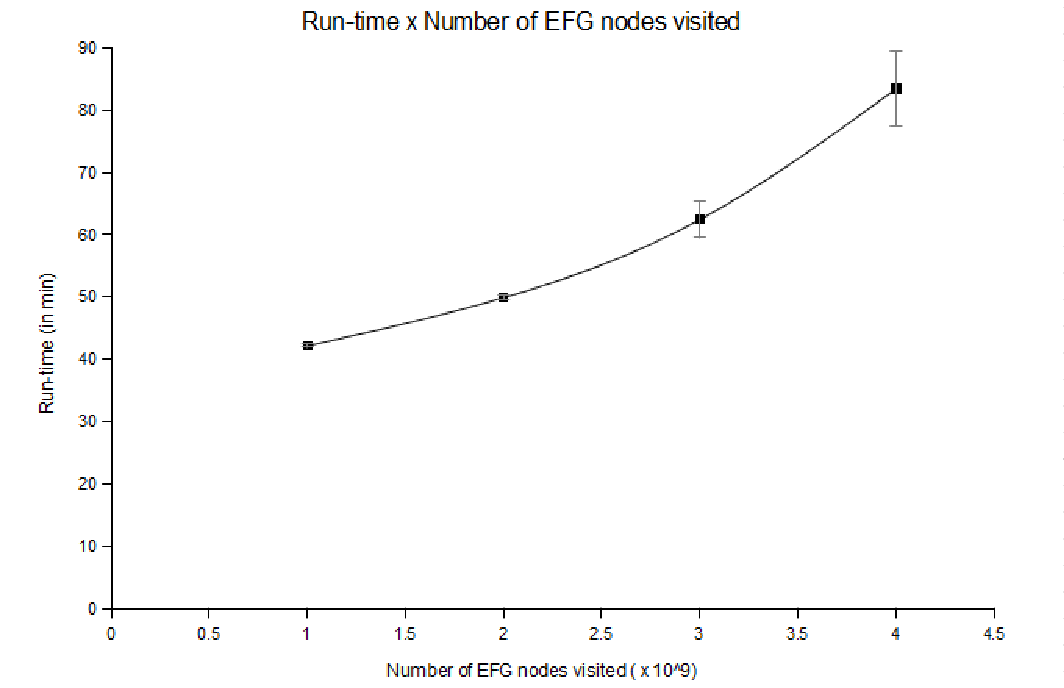
\includegraphics[scale=0.3]{figures/plot1.eps}
    \caption{Plot 1 description.}
    \label{fig:Plot1}  
\end{figure}

\begin{figure}[h!]
\centering
    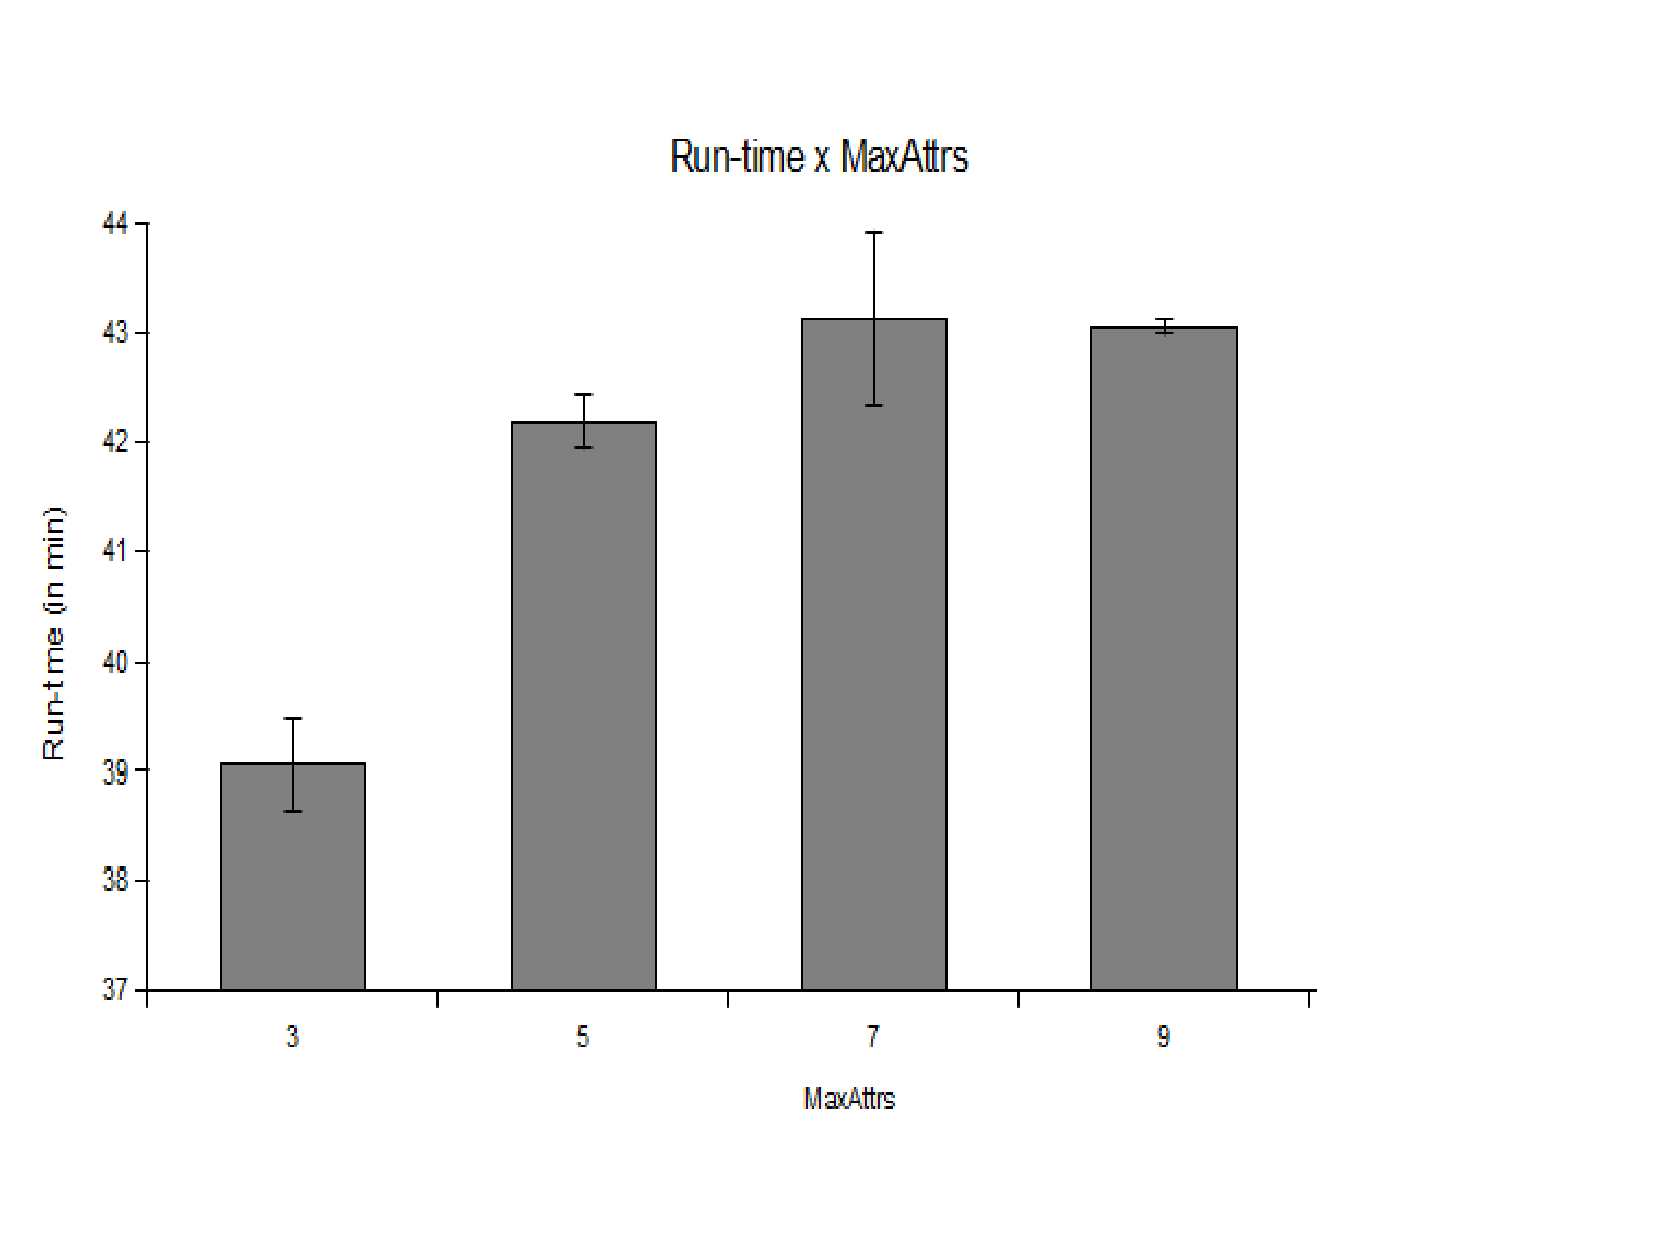
\includegraphics[scale=0.3]{figures/plot2.eps}
    \caption{Plot 2 description.}
    \label{fig:Plot2}  
\end{figure}


\section{The AFGMiner Algorithm}
	\label{sec:AFGMiner}
	AFGMiner generates and tests candidate patterns of increasing number of edges, then extends those patterns considered heavyweight. It generates candidate patterns of $k$ edges, starting with $k = 0$ (patterns composed of a single node and no edges), and searches for occurrences of such patterns in the dataset by using a sub-graph isomorphism detection algorithm. Each ocurrence found has its node weight and edge weight support values computed, and, when no more occurrences of a pattern are present in the dataset, the support value for the pattern itself is computed by aggregating the support values of its occurrences. If the support value for the pattern is higher than an user-defined threshold, the pattern is heavyweight. It is then output to the user and later extended into candidate patterns with an additional edge, a process called \emph{edge-by-edge pattern extension}. If the pattern is not heavyweight, it is discarded. 

Edge-by-edge pattern extension works by adding to a pattern either: (i) an edge that connects two of its nodes; (ii) or an edge that connects one of its nodes to a new node called the \emph{extension node}. A pattern that generates other patterns by extension is called a \emph{parent pattern}, while the generated patterns are \emph{child patterns}.

\subsection{Canonical Labeling}
It is possible that two different patterns, when extended, generate child patterns that are isomorphic. It is inefficient to mine for redundant patterns, so redundancy should be detected. The well-known concept of \emph{canonical labeling} of patterns is used to detect redundancy~\cite{gSpan}. The idea is to map each sub-graph pattern to an identifier string called \emph{DFS Code}. The string representation, or DFS Code of an AFG of $n$ edges is $(e_0) (e_1)...(e_n)$, where each edge $e_i=(v_i, v_j)$ is represented by a string: $( [l(v_i):$ $(a_{i_0})$ $(a_{i_1})...(a_{i_m})]$ $[l(v_j): (a_{j_0}) (a_{j_1})...(a_{j_p})] )$, where $m$ and $p$ are the number of attributes present in the edge's \emph{from-node} and \emph{to-node}, respectively. DFS Codes can be lexically ordered in such a way that, if two sub-graphs are isomorphic to each other, they provably have the same minimum DFS Code. The rules that define how to sort DFS Codes depend on the types of graphs being mined. 

In order for a newly-generated sub-graph pattern to be considered redundant, and thus discarded, its DFS Code should be already present in $H$, a hash-set whose elements are the distinct DFS Codes of all patterns that have been processed. However, this approach may consume large amounts of memory because the number of candidate patterns generated may be very high. Instead, the approach adopted in the prototype implementation of AFGMiner is to record the DFS Codes only for patterns considered heavyweight. 

When producing the DFS Code of a sub-graph pattern, it is a requirement to label the edges and nodes of the pattern. Nodes are labelled as follows. The attribute set of the node is used as its preliminary label, by forming a bit vector in which each attribute is represented by a bit presence or absence of the attribute. Edge labels are simply the labels of the edges's \emph{from-node} and \emph{to-node} in that order. The edge labels are sorted by considering that, given any two edge labels, the one with the lower \emph{from-node} label comes first, and in case those are the same, the one with the lower \emph{to-node} label comes first. The minimum DFS spanning tree of the sub-graph pattern is then computed using the sorting order of the edge labels \emph{in lieu} of edge weights. Finally, the order in which pattern nodes are visited during a pre-order traversal of this minimum spanning tree determines their final and unique-per-pattern label, which is used to sort the edges. The resulting sorted edge labels of two patterns is the same if the patterns are isomorphic.

\subsection{Support Value Policy}
The process of generating and testing candidate patterns in AFGMiner may be understood as the exploration of the space of patterns that exist in the dataset of AFGs being mined. The algorithm searches for all the heavyweight patterns present in this space, which can be envisioned as a forest of trees with the root node of each tree being a 0-edge pattern, child nodes of the root node being the 1-edge patterns extended from the 0-edge patterns, etc. Pruning this search space as much as possible is desirable in order to decrease the run-time of the algorithm. AFGMiner adopts an \emph{anti-monotonic} support value policy to enable the pruning of the search space. Under this policy, the support value of a pattern is always lower than or equal to the support value of any of its ancestor patterns. Therefore, if a pattern is not heavyweight, none of its descendants can be heavyweight. Thus all patterns that do not meet a minimum support criteria can be discarded. The anti-monotonic support value policy allows the algorithm to prune  nodes in the search space that it identifies as non-heavyweight patterns. 

The support value policy works as follows. For each occurrence $g$ of a pattern $p$, two values are calculated: $S_n(g)$, the weight of the attribute with minimum weight amongst all attributes associated with nodes of $g$; and $S_e(g)$, the minimum edge weight amongst all edges of $g$. The $S_n(g)$ of all occurrences of $p$ found in $DS$ are then added up, resulting in $S_n(p)$, the node weight support of $p$. The $S_e(g)$ of all occurrences of $p$ found in $DS$ are also added up, resulting in $S_e(p)$, the edge weight support of $p$. The support value for $p$ is $S_m(p)$, the maximum between $S_n(p)$ and $S_e(p)$. $S_m(p)$ is compared against the support threshold to decide whether $p$ is a heavyweight pattern. 

The principle behind separately computing the support values of node attributes and edges of a pattern and then choosing the maximum between the two values is that a pattern is relevant if either, or both, the attributes or edges of its occurrences have significant weight in comparison to the sum of all node weights and to the sum of all edge weights in the dataset. The support-value policy selected for AFGMiner is conservative because only the minimum edge weight and the minimum node attribute weight of each occurrence are used in the computation. Less conservative support-value policies could be adopted as long as they are anti-monotonic.  

\subsection{Matching Patterns to Occurrences}
When a candidate pattern is generated, its DFS Code is computed and the algorithm checks if the DFS Code already exists in $H$. If the DFS Code is not present, the candidate pattern is not redundant and the process of mining for it in the dataset begins. The mining process finds sub-graphs $g$ in AFGs of $DS$ that match the candidate pattern $p$. AFGMiner may use any sub-graph isomorphism detection algorithm to match patterns and sub-graphs, as long as the algorithm is adapted to take node attributes into consideration when detecting isomorphism. The prototype implementation of AFGMiner adapts VF2~\cite{Cordella}, an algorithm that is faster than alternatives for graphs that are relatively regular, have a large number of nodes and whose nodes have small valency~\cite{Foggia}. For the case study described in this paper, AFGs meet this criteria. 

VF2 produces a mapping $M$ between nodes in $p$ and nodes in $G$, where $G$ contains at least as many nodes as $p$. $M$ is expressed as a set of pairs $\{n, m\}$, where $n \in p$ and $m \in G$ are nodes. The mapping is said to be an isomorphism if $M$ is a bijective function that preserves the branch structure of both $p$ and $G$. This mapping is represented as a state $s$ in a State Space Representation (SSR). This state, which we call a \emph{miner state}, goes from empty (no mapping between nodes in $p$ and nodes in $G$) to a goal state (all nodes in $p$ mapped to respective nodes in $G$) during the process of finding $M$. A state transition between any miner state $s_1$ and its successor $s_2$ represents the addition of a new pair $\{n, m\}$ to the collections of known pairs that compose $M$. The addition of new pairs only occurs if $n$ and $m$ form a feasible pair. The rules for a pair of nodes to be considered feasible, in the case of AFGs, are as follows: (i) attributes of $m$ should be a proper superset of attributes in $n$; (ii) topological structure around $n$ and $m$ should be the same.

\subsection{Generation of Candidate Patterns}
The input to AFGMiner is a list $A_0$ of attributes that occur in the dataset. Each one of the possible attributes is used to create a set of 0-edge candidate patterns with a single attribute in their nodes, as shown in Figure~\ref{fig:example_0-edge}. The support value threshold in this example is $T = 1/23$. Each one of the candidate patterns $p$ is mined for in the dataset $DS$, and, if $p$ is heavyweight, its only attribute is added to $A_1$. $A_1$ is the list of distinct attributes that belong to 0-edge heavyweight patterns and that are used in the generation of 1-edge candidate patterns. 

After all 0-edge heavyweight patterns of a single attribute are found, the attributes in $A_1$ are combined in pairs and AFGMiner searches for the generated 0-edge candidate patterns that have two attributes each (Figure~\ref{fig:example_0-edge_2-attribute}). The attributes that compose the 0-edge candidate patterns of two attributes found to be heavyweight are then combined into sets of three attributes, which form the 0-edge candidate patterns of three attributes each. This continues until no more 0-edge heavyweight patterns with a certain number of attributes can be found. 

The process of mining for candidate patterns with an increasing number of attributes in their single node (in the case of 0-edge patterns) or in their extension node (in the case of $k$-edge patterns with $k > 0$) is called \emph{attribute-set growth}. Attribute-set growth is useful because an attribute set is only used to generate a pattern if all of its sub-sets generated heavyweight patterns. 

Each one of the 0-edge heavyweight patterns spans multiple child candidates, one for every attribute in $A_1$, in which the extension node contains a single attribute from $A_1$. Thus, all the pairs of nodes connected by an edge in Figure~\ref{fig:example_1-edge} are child candidates for the example. AFGMiner searches for matches for each candidate child pattern in the dataset as soon as the pattern is generated. If a candidate pattern is found to be heavyweight, all its attributes are added to $A_2$. Attributes in $A_2$ are then used to generate 1-edge candidate patterns that have two attributes in their extension node.  In Figure~\ref{fig:example_1-edge_2-attribute} a candidate is generated for each pair of nodes connected by an edge. For clarity, only candidates generated by the pattern $a$ $\rightarrow$ $a$ are shown. The attribute-set growth process then proceeds until no more 1-edge candidate patterns of certain number of attributes in their extension node can be found. In Figure~\ref{fig:example_2-edge}, 2-edge patterns are shown. 

A set of patterns that have the same number of edges is called a \emph{generation}. AFGMiner produces and mines for candidate patterns generation by generation as described above. Patterns of a certain generation are only created and mined after all the heavyweight patterns of the previous generation have been found. This is important because it allows the algorithm to use only the $A_k$ set of distinct attributes present in the $(k - 1)$-th generation to compose the patterns of the $k$-th generation, thus restricting the number of candidate patterns produced.

\begin{figure}[h!]
\centering
    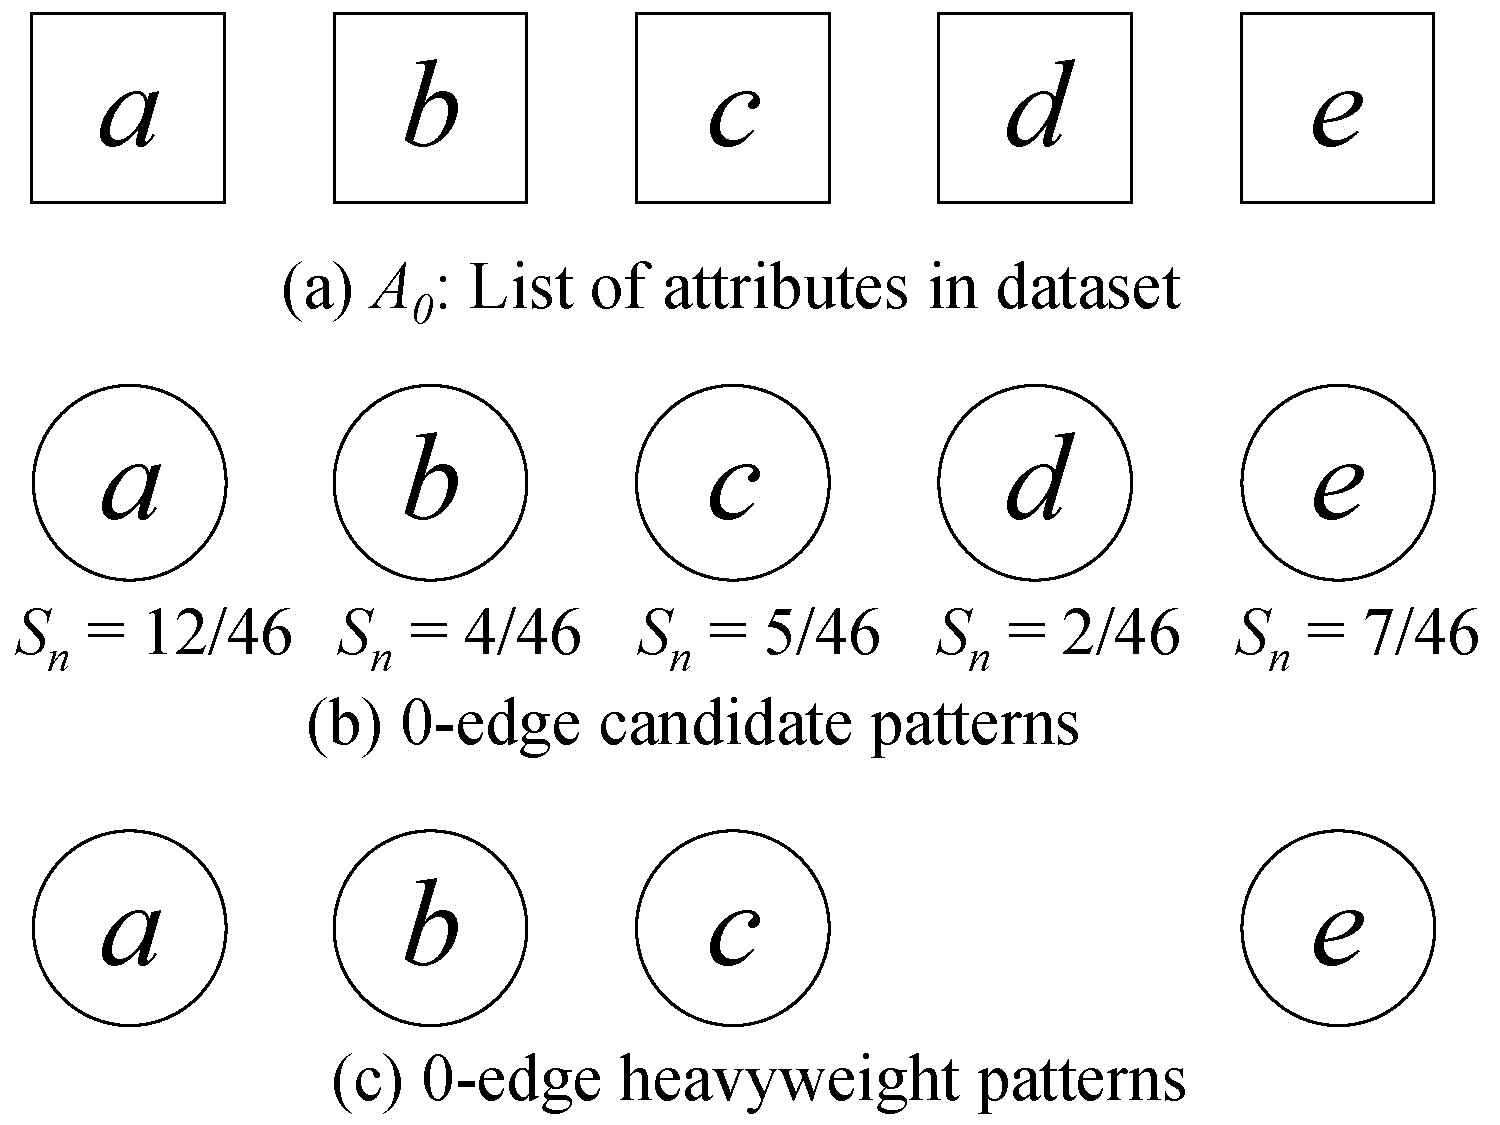
\includegraphics[scale=0.15]{figures/example_0-edge.pdf}
    \caption{0-edge candidate patterns.}
    \label{fig:example_0-edge}  
\end{figure}

\begin{figure}[h!]
\centering
    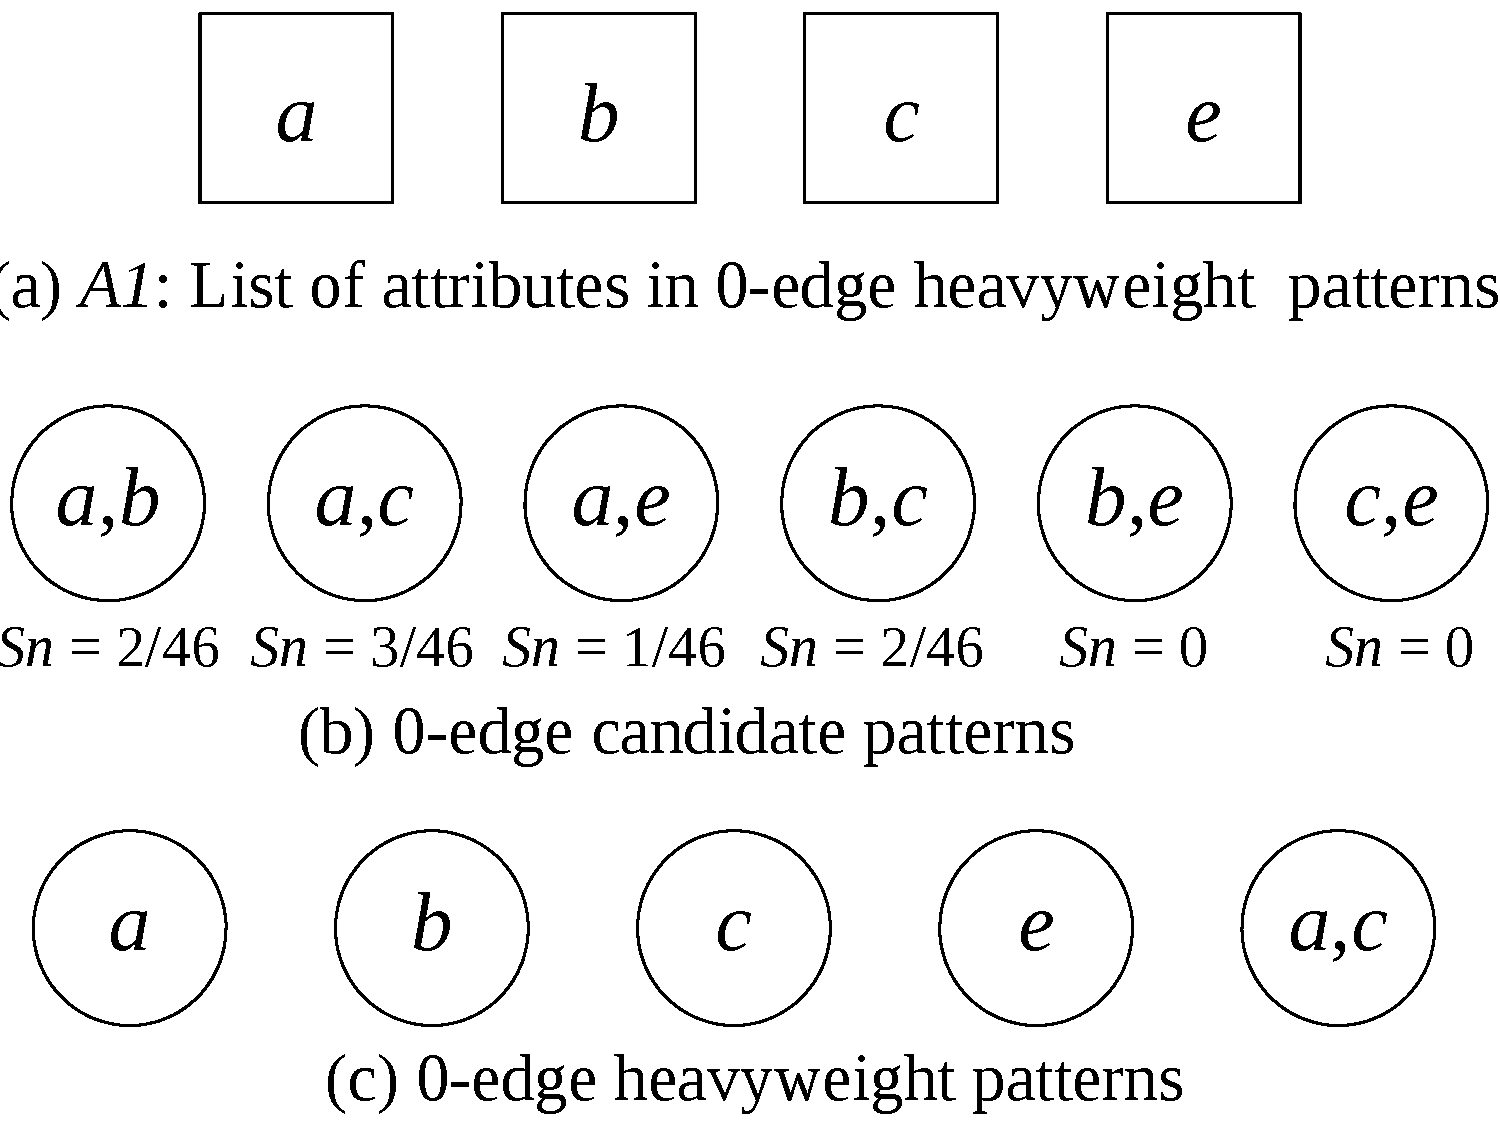
\includegraphics[scale=0.15]{figures/example_0-edge_2-attribute.pdf}
    \caption{Attribute-set growth for 0-edge candidate patterns.}
    \label{fig:example_0-edge_2-attribute}  
\end{figure}

\begin{figure}[h!]
\centering
    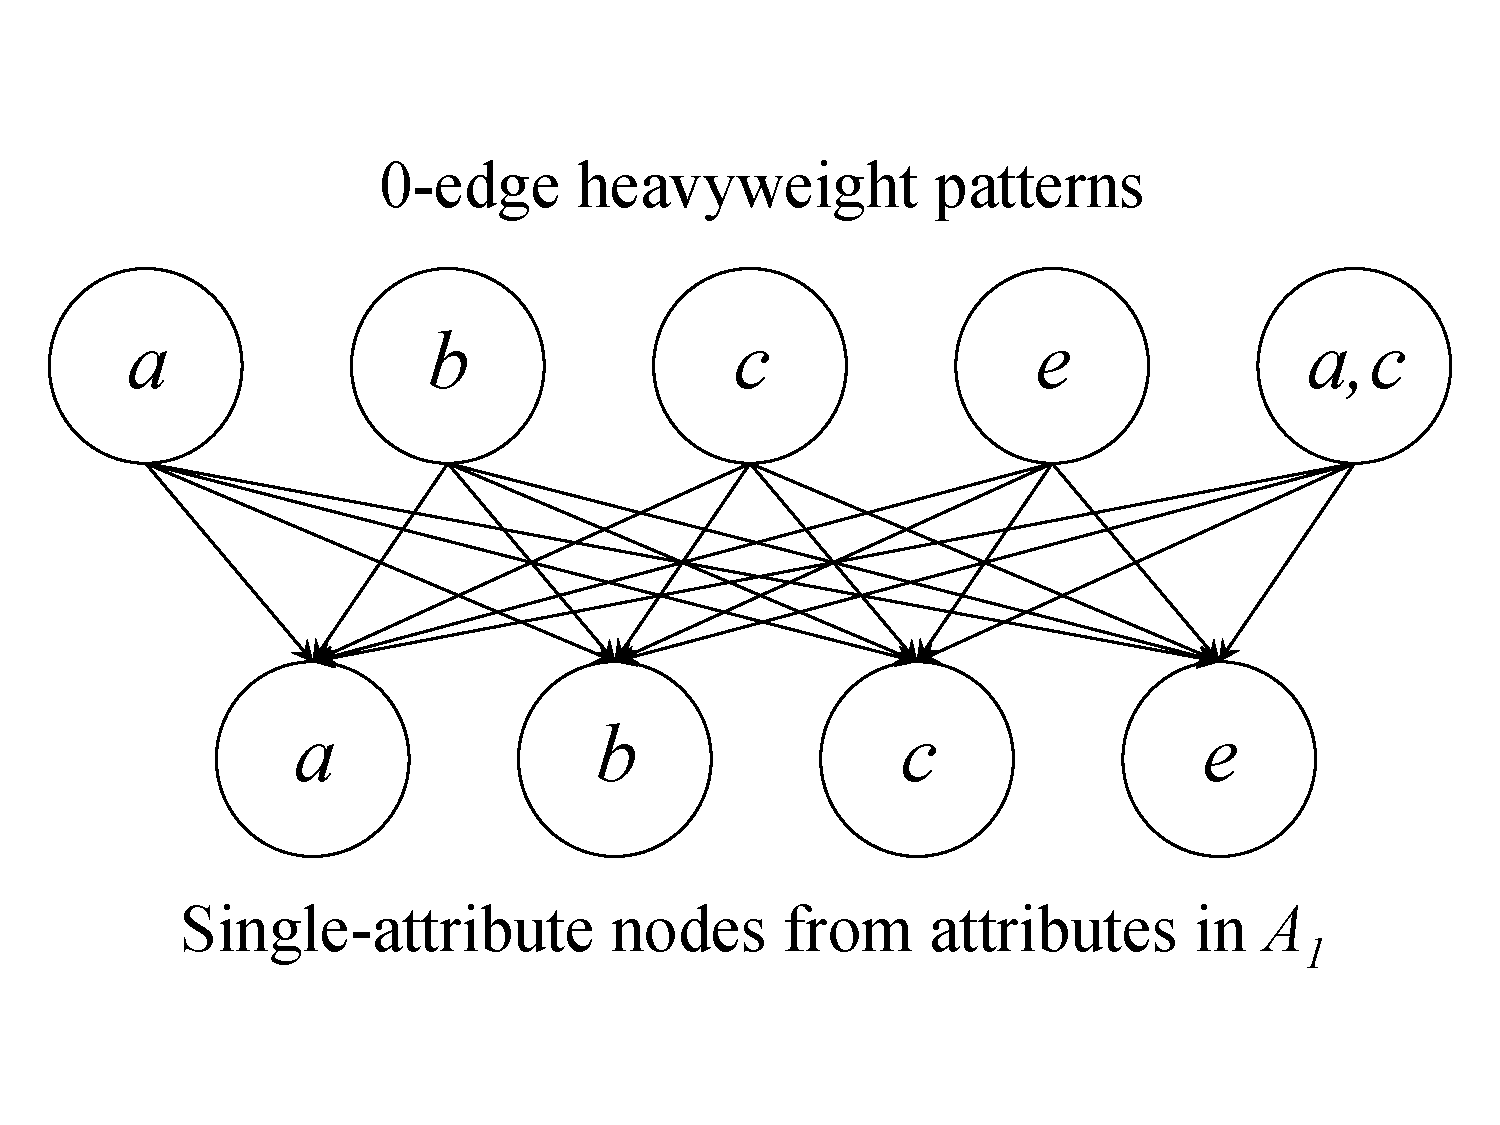
\includegraphics[scale=0.15]{figures/example_1-edge.pdf}
    \caption{1-edge candidate patterns.}
    \label{fig:example_1-edge}  
\end{figure}

\begin{figure}[h!]
\centering
    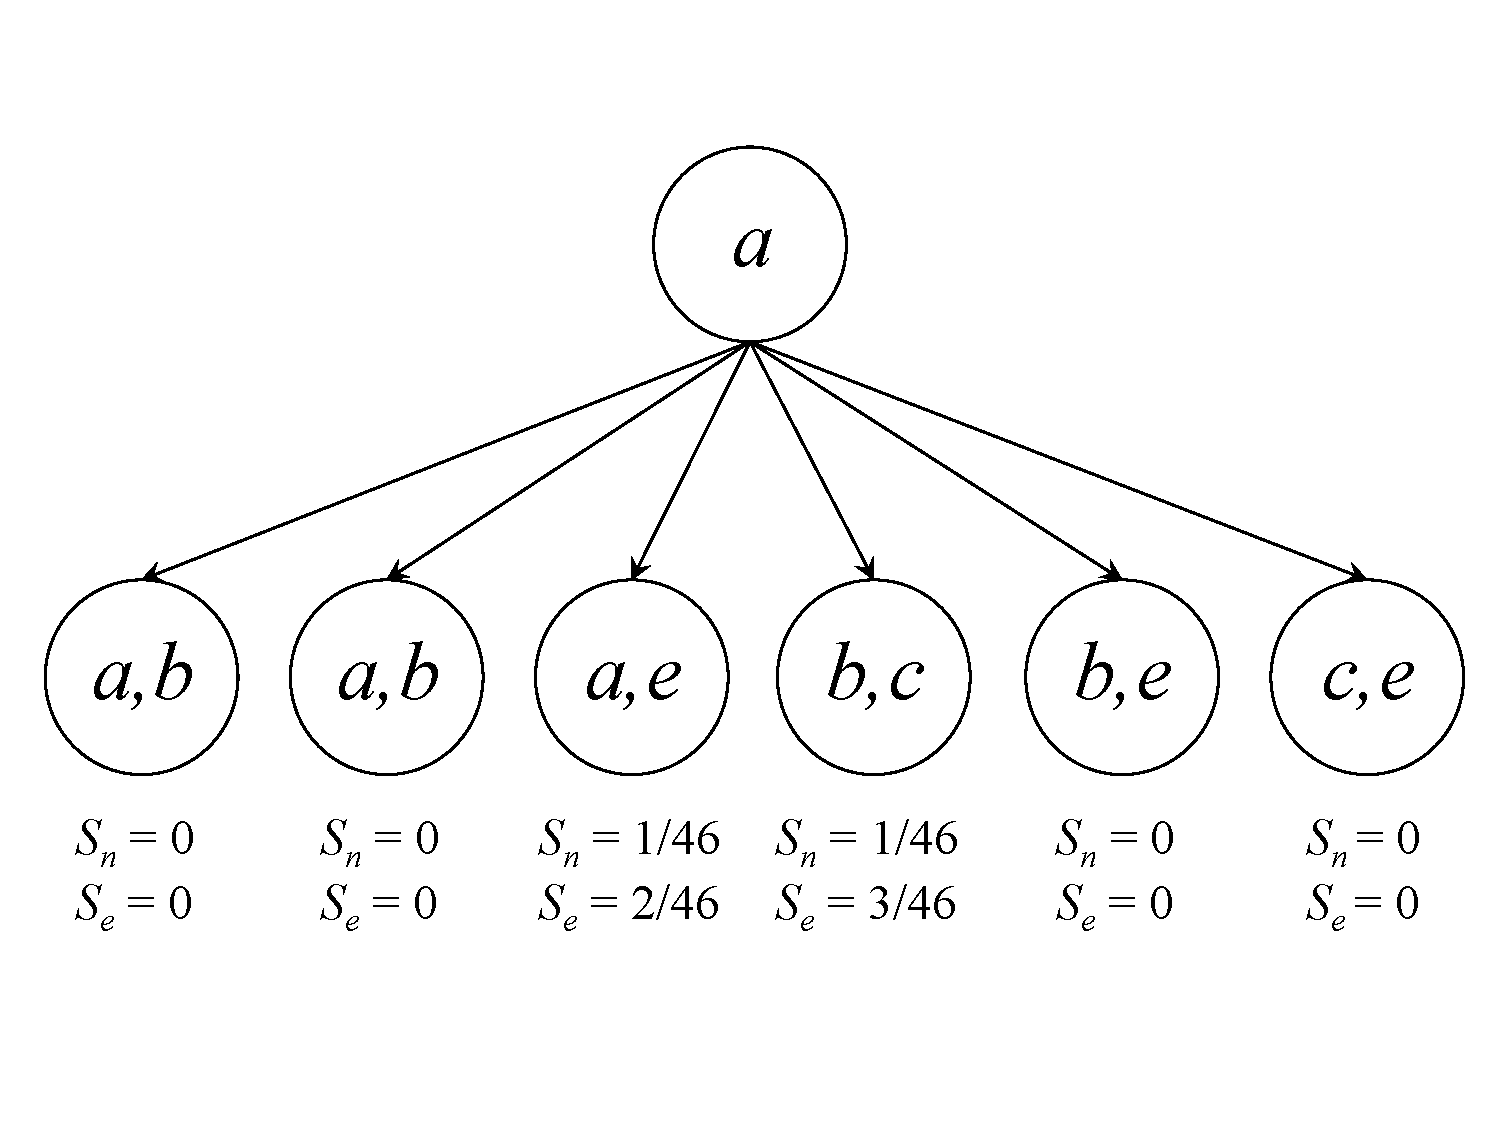
\includegraphics[scale=0.15]{figures/example_1-edge_2-attribute.pdf}
    \caption{Attribute-set growth for 1-edge candidate pattern node $a$ $\rightarrow$ $a$. }
    \label{fig:example_1-edge_2-attribute}  
\end{figure}

\begin{figure}[h!]
\centering
    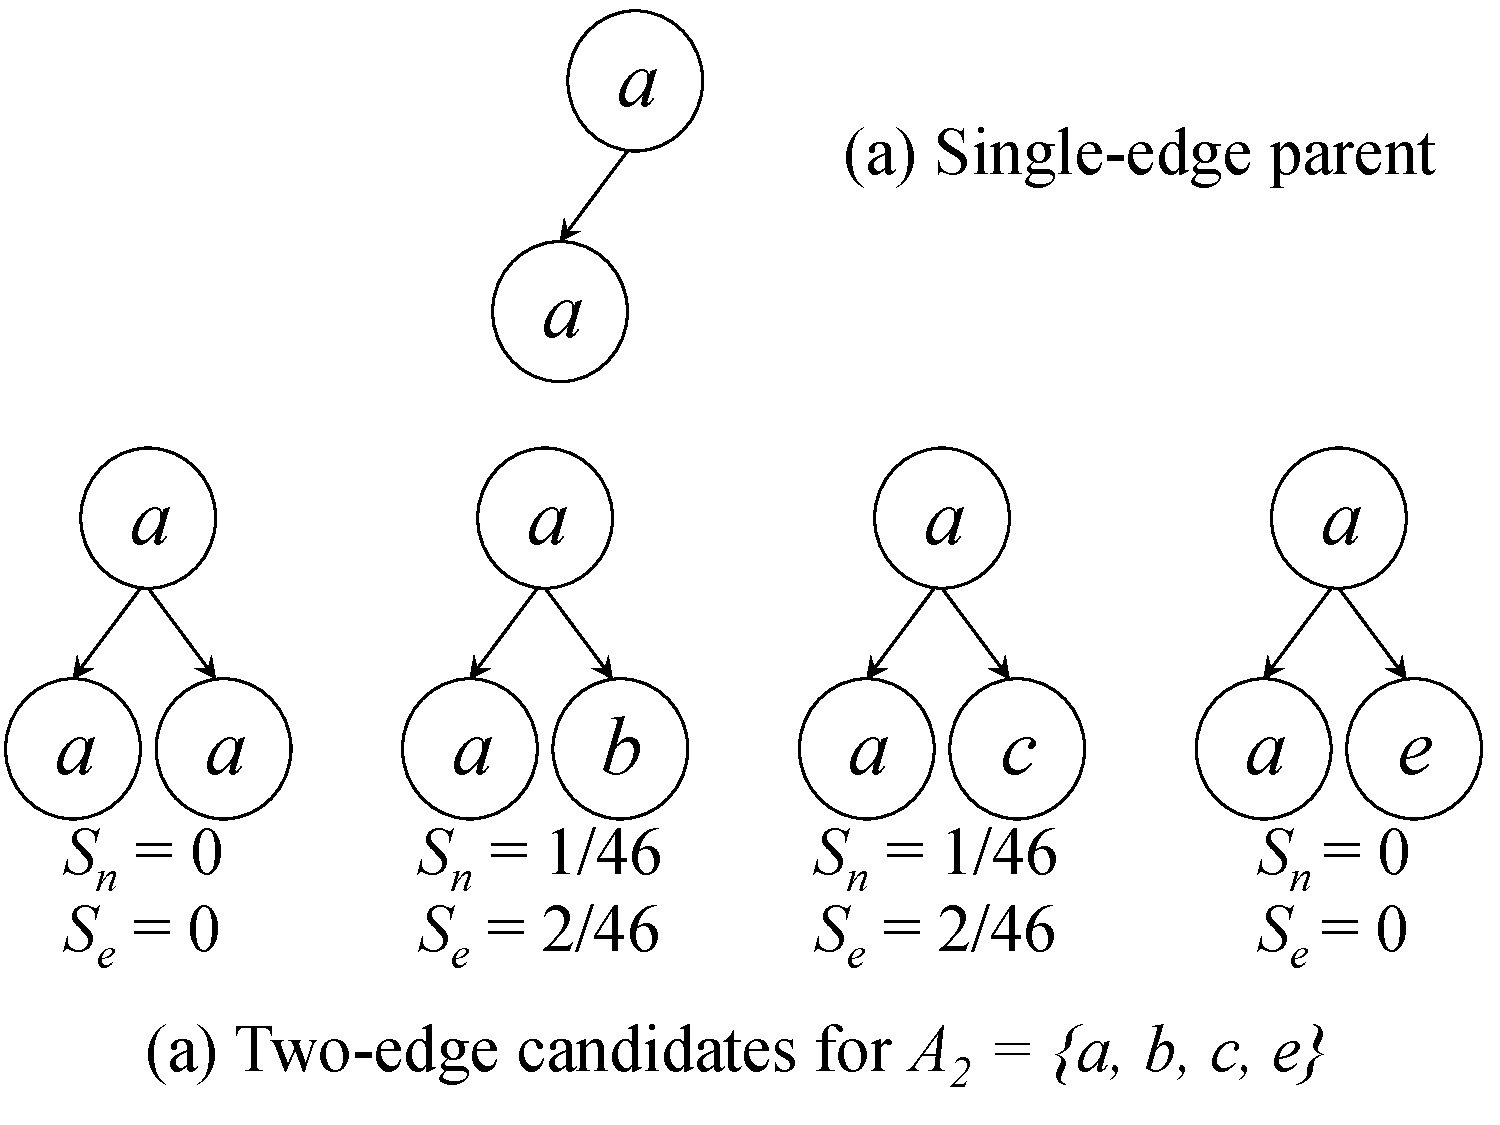
\includegraphics[scale=0.15]{figures/example_2-edge.pdf}
    \caption{2-edge candidate patterns.}
    \label{fig:example_2-edge}  
\end{figure}



\section{Algorithm Improvements}
	\label{sec:Improvements}
	The previous section described the original version of AFGMiner, called {\bf AFGMiner-iso} (\emph{iso} stands for isomorphism detection). AFGMiner-iso visits all nodes in the dataset for every pattern searched, making it potentially slow when analyzing large datasets composed of thousands of AFGs with hundreds of nodes each, as in the case study presented in this work. Another version of AFGMiner, {\bf AFGMiner-locreg}, addresses this performance issue. It uses the concept of location registration.

{\bf Location Registration} is the complete mapping, including nodes and edges, between a candidate pattern $p$ and each of its occurrences $g$. If $p$ is found to be heavyweight, this mapping is kept, otherwise it is discarded. Then, when a heavyweight pattern $p$ is extended into its child patterns $c$, in order to find occurrences of $c$ the algorithm only checks the mappings between $p$ and its occurrences $g$. In order to generate $c$, $p$ has one of its nodes, $v$, extended by adding to it an edge $e$, and may also have an extension node $q$ connected to $e$. The idea of location registration is to check each mapping between $p$ and occurrences $g$ for: (i) the node $v_g$ in $g$ that corresponds to $v$; (ii) if $v_g$ is connected to an edge $e_g$ that corresponds to $e$ and (iii) in case $c$ was extended from $p$ by adding an extension node, check if $e_g$ connects a node $q_g$, corresponding to node $q$, to $v_g$. If the algorithm is able to find appropriate $v_g$, $e_g$ and $q_g$ attached to the occurrence $g$, then the sub-graph that is composed of $g$ plus $e_g$ and $q_g$ is an occurrence of $c$.







        \subsection{A Parallel Implementation of AFGMiner}
	\label{sec:pAFGMiner}
	A parallel version of AFGMiner benefits from the multiple cores available in many computing systems. An important challenge in the implementation of a parallel version of AFGMiner-locreg, {\bf p-AFGMiner}, is the distribution of the workload to improve load balancing.

p-AFGMiner executes the following steps while a queue $Q$ of heavyweight patterns is not empty (s signals a sequential step, while p signals a parallel step): (i-s) fork into $n$ threads to start the processing of a new generation composed of patterns with $k$ edges.

For $k = 0$, (ii-s) divide the set $A_0$ among the threads and (iii-p) each thread generates 0-edge candidate patterns using their part of $A_0$ and searches the database for these patterns --- heavyweight patterns form a local queue $Q_{TL}$ and the set of attributes in $Q_{TL}$ form $A_{TL}$, the local set of attributes.

For $k > 0$, (ii-s) distribute the queue $Q$ of $k$-edge heavyweight patterns among $n$ thread-local queues $Q_{TL}$; (iii-p) each thread generates $(k+1)$-edge candidates from patterns in $Q_{TL}$ and computes their support, generating $A_{TL}$ and adding the patterns found to be heavyweight to $Q_{TL}$; 

Then: (iv-s) synchronize when all threads finish step (iii) and unify all $Q_{TL}$s into a single queue $Q$, and all $A_{TL}$s into a single $A_{k+1}$ set of attributes; and (v) start processing the next generation, if $Q$ is not empty. The dataset of AFGs, $DS$, is read-only during the entire run of p-AFGMiner, allowing the maintenance of thread-local versions of variables and thus reducing synchronization.

The distribution of $Q$ among threads should balance the workload to improve the performance of p-AFGMiner. The number of occurrences of the parent of a pattern $p$ in $DS$ is the most important factor determining the time required to search for occurrences of $p$. A reasonable heuristic tries to balance the number of parent-pattern occurrences assigned to each thread. 

\begin{figure}[h!]
\centering
    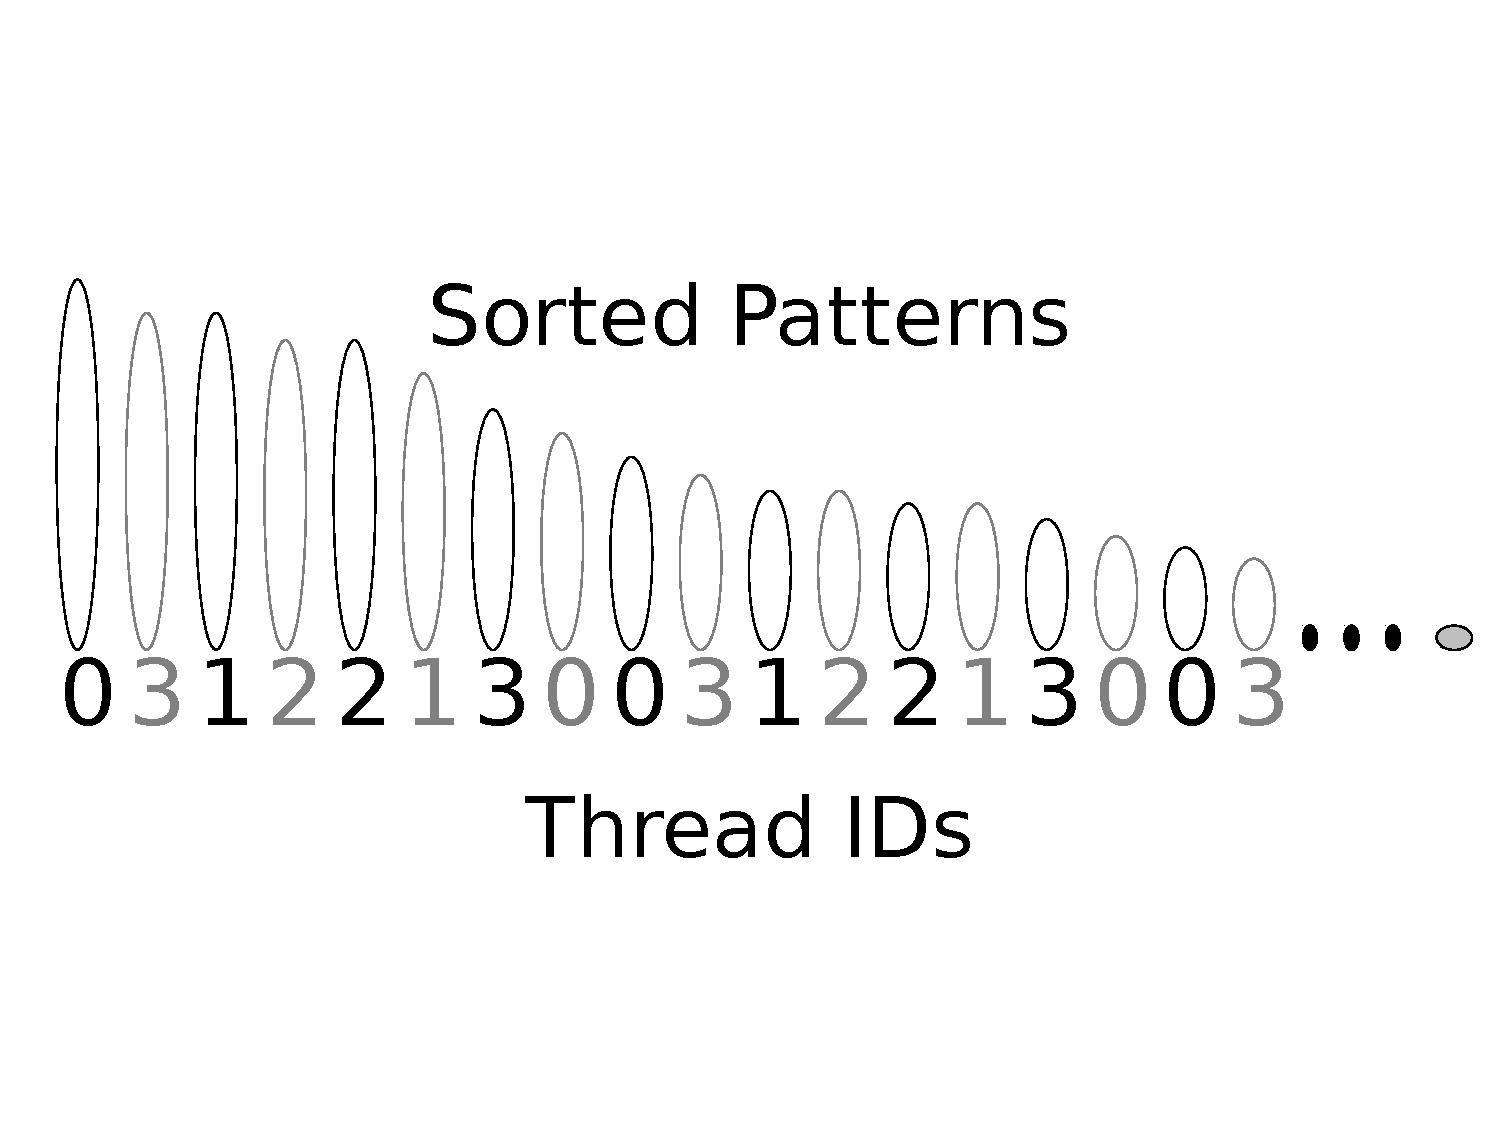
\includegraphics[scale=0.3]{figures/WorkDistributionHeuristic.pdf}
    \caption{Illustration of pattern distribution heuristic.}
    \label{fig:WorkDistributionHeuristic}  
\end{figure}

The pattern-distribution heuristic created for p-AFGMiner sorts the $m$ patterns in $Q$ by decreasing order of the number of parent-pattern occurrences. The heuristic then does a round-robin assignment of patterns to threads following an increasing order for the patterns with an even position in the sorted $Q$ and in decreasing order for patterns with an odd position in the sorted $Q$ as illustrated in Figure~\ref{fig:WorkDistributionHeuristic} --- assume that numbering in $Q$ starts at zero. In this illustration each ellipse represents a pattern in $Q$ and the size of the ellipse stands for the number of occurrences of the pattern's parent in the database.
This simple $O(n)$ heuristic is effective for a moderate number of threads and for limited variations in the number of parent-pattern occurrences. Experimental evaluation revealed that this workload-distribution heuristic lowered the execution time of p-AFGMiner, on average, by 6\% when compared with a naive workload distribution method that simply distributes patterns among the threads without any sorting.


 


 

	
\section{Case Study: Using AFGMiner for Program Analysis}
	\label{sec:CaseStudies}
	The  {\bf Profile-based Program Analysis} (PBPA) problem, a common challenge among compiler engineers and computer architects, is defined as follows. Given a profile {\em Prof} obtained from an execution of a computer program, automatically discover operation patterns in the execution of {\em Prof} that, in aggregation, account for a sufficiently large fraction of the program's execution time. If PBPA is properly handled, developers are then able to focus their optimization efforts on those areas in the program code that correspond to occurrences of the relevant operation patterns. In order to solve PBPA, we convert it to a heavyweight pattern mining problem, by modeling the program as a dataset of attributed flow graphs named \emph{Execution Flow Graphs} (EFGs). EFGs are control flow graphs with added attributes (hardware-related events captured by performance counters) and associated weights (CPU cycles spent on instructions and events). Our tool HEPMiner then uses the AFGMiner algorithm to find \emph{heavyweight execution patterns} (HEP): sets of hardware-related events associated with assembly instructions that were executing when the events happened~\cite{GomesMSc12}.

\subsection{Sub-Graph Mining in Bounded Treewidth Graphs}

Tree-width is a measure of how similar to a tree a graph is. It is a very useful property because several NP-hard problems on graphs become tractable for the class of graphs with bounded tree-width, including sub-graph isomorphism detection and, as a consequence, frequent sub-graph mining of connected graphs~\cite{Horvath}. \emph{Horvarth and Ramon} discovered a level-wise sub-graph mining algorithm that lists frequent connected sub-graphs in incremental polynomial time in cases when the tree-width of the graphs being mined is bounded by a constant~\cite{Horvath}. In addition, \emph{Thorup} shows that graphs representing the control flow of structured programs (\ie CFGs) have tree-width of at most six~\cite{Thorup}.  Since EFGs have the same topology as CFGs, they also have bounded tree-width. Thus, when applied to the PBPA problem, AFGMiner runs in incremental polynomial time because the problem being solved is fundamentally finding frequent connected sub-graphs in a dataset of EFGs. The addition of weights in nodes and edges and weighted attributes to nodes does not change the complexity of the algorithm, but the generation of attribute sets of increasing size when creating new candidate patterns could. However, the number of attributes that an extension node of a $k$-edge candidate pattern with $k > 0$, or that the single node of a 0-edge candidate pattern, can have is bounded by the size of $A$, \ie by the number of possible attributes that each pattern node may contain. As a consequence, the attribute-set growth component of the algorithm has a constant complexity, while the sub-graph mining component has incremental polynomial complexity.



	\subsection{A Tool for Compiler Developers and Computer Architects}
		\label{sec:HEPMiner}
		HEPMiner is a program performance analysis tool that requires information about the static control flow of the program and its behavior at run-time. Dynamic information about the program is obtained by profiling its methods and includes which instructions are executed and which hardware events are triggered as a result of instruction execution. When the program is profiled, compiler log files (typically one per running thread) are created with edge profiling information, \ie basic blocks and flow edges of each method and their execution frequency measured in CPU cycles. A hardware profile is also generated and contains sequences of instructions and associated hardware events, captured by performance counters during run-time. Each instruction has a corresponding number of cycles during which it was executed, and the number of cycles in which each event was active. 

The information from compiler log files and hardware profile goes into database tables later read by HEPMiner, that assembles one EFG per profiled method. An EFG node is created for each assembly instruction in the profile; instructions in the same basic block are connected by new flow edges and the frequency of such edges is the same as the frequency of those basic blocks that they connect. The nodes at the end of each basic block are connected to the first nodes of all subsequent basic blocks as determined by edges in the CFG of the method, and the frequency of these edges is set to the frequency of the corresponding CFG edges. The weight of each EFG node is the number of sampling ticks associated with the corresponding assembly instruction that the node represents, and the attributes of a node are the attributes associated with the same instruction. Performance counters can mostly be directly converted into attributes. 

With all EFGs assembled, HEPMiner uses the AFGMiner algorithm to find \emph{heavyweight execution patterns} (HEP). HEPs are sets of hardware-related events captured by performance counters and associated with assembly instructions that were executing when the hardware-related events happened. Examples of such events are the occurrence of instruction and data cache misses, directory misses, address-generation interlocks. All these events that happen at program run-time result from effects that the assembly instructions being fetched, decoded and executed have on the pipeline of instructions, and from the interactions between such instructions and data that they load and store to and from caches and memory. These events affect program performance and it is thus important for compiler and architecture developers to understand when and why they happen, and which sets of events, correlated with which sets of instructions, take up more execution time. If the profile of a program is flat, manually searching for time-consuming correlations between hardware events and instructions becomes a challenge. HEPMiner automates this process, and finds non-obvious correlations represented by execution patterns that take up significant execution time when their occurrences are considered in aggregation.

		
\section{Performance Evaluation Methodology}
	\label{sec:Methodology}
	Experiments for HEPMiner were performed on an Intel Core 2 Quad CPU Q6600 machine, running at 2.4 GHz and with 3 GB of RAM.

\subsection{HEPMiner Evaluation}
The experimental evaluation of the algorithm in the context of HEPMiner uses profiles from the DayTrader Benchmark, running on IBM's WebSphere Application Server, on an IBM z196 mainframe~\cite{zEnterprise} and JIT-compiled using the IBM Testarossa JIT compiler. The WebSphere Application Server is a Java\textregistered~Enterprise Edition (JEE) server~\cite{WAS}. It has a very flat profile, with its execution time spread relatively evenly over 2,566 methods, as is typical of large business applications.

Four experiments examine the performance trends of AFGMiner: {\bf A}, {\bf B}, {\bf C} and {\bf D}, described in more detail below. All experiments were run on DayTrader methods that were profiled using hardware instrumentation. Three important parameters in the experiments are: the minimum support threshold (MinSup) and the maximum allowed size of the attribute set in each candidate pattern node (MaxAttrs), both described in Section~\ref{sec:ProblemDef}; and the \emph{Minimum Hotness Method} (MMH) value. The MMH is calculated by dividing the sum of all CPU cycles associated with each one of DayTrader's profiled methods by the cycles associated with the entire program run. This parameter is used in the experiments simply to limit the methods analyzed by the algorithm to those that contribute most significantly to total program run-time, and are thus more likely to contain patterns of interest to compiler engineers. 

For experiments {\bf A}, {\bf B} and {\bf C}, the MMH is kept at 0.001, meaning that only methods with execution time that exceeds 0.1\% of program run-time are selected for mining (\emph{i.e.} in DayTrader, 278 of 2,566). For experiment {\bf D}, the MMH has values 0.001 (278 methods), 0.003 (56 methods) and 0.005 (23 methods). For all experiments except {\bf A}, MaxAttrs is kept at 5.

\emph{Experiment {\bf A}} compares the run-times of AFGMiner-locreg with respect to changes in MaxAttrs. MinSup is kept at 0.001, meaning that only those patterns consuming more than 0.1\% of program run-time are considered heavyweight. Increasing MaxAttrs potentially causes more candidate patterns to be generated, which is why modifying this parameter is a way of controlling the memory consumed by the algorithm and also its run-time. 

\emph{Experiment {\bf B}} compares the run-times of AFGMiner-locreg with respect to changes in the number of EFG nodes visited by the algorithm. The number of EFG nodes visited is controlled by changing MinSup.

\emph{Experiment {\bf C}} compares run-times of AFGMiner-locreg and p-AFGMiner with 2, 4, 6 and 8 threads, by changing MinSup.

\emph{Experiment {\bf D}} compares run-times of AFGMiner-locreg and p-AFGMiner with 2, 4, 6 and 8 threads by changing MMH. MinSup is kept at 0.001.

Patterns found by AFGMiner-locreg were also compared to the ones found by the FlowGSP algorithm. FlowGSP was modified to support variations in MMH, MinSup and MaxAttrs, and run on DayTrader methods with the same parameter values used for Experiment {\bf B} above. In addition, expert compiler engineers from IBM's JIT Compiler Development team verified the usefulness of patterns identified by the HEPMiner tool, as described in Section~\ref{sec:QualAnalysis}.









\section{Performance Evaluation}
	\label{sec:PerformanceEvaluation}
	In our experiments using HEPMiner, AFGMiner-locreg was always faster than AFGMiner-iso. As an example, when running with MMH and MinSup of 0.001, AFGMiner-iso took approximately 11 hours to complete the mining process, while AFGMiner-locreg took 40 minutes and p-AFGMiner with 8 threads took 15 minutes. The dramatic decrease in run-time when comparing AFGMiner-locreg to AFGMiner-iso is expected because location registration decreases the number of dataset sub-graphs that must be tested for isomorphism with candidate patterns. 

We also compared patterns found by AFGMiner and FlowGSP. Figure~\ref{fig:NumPatterns} shows the number of output patterns for different MinSup values. As expected, AFGMiner found all patterns found by FlowGSP, but also found additional patterns composed of multiple sub-paths. For flat profiles, the trend is for AFGMiner to find many more patterns than FlowGSP as the MinSup is decreased, with the sequential patterns found by both being the parent patterns of the sub-graph patterns found exclusively by AFGMiner. 

\begin{figure}[h!]
\centering
    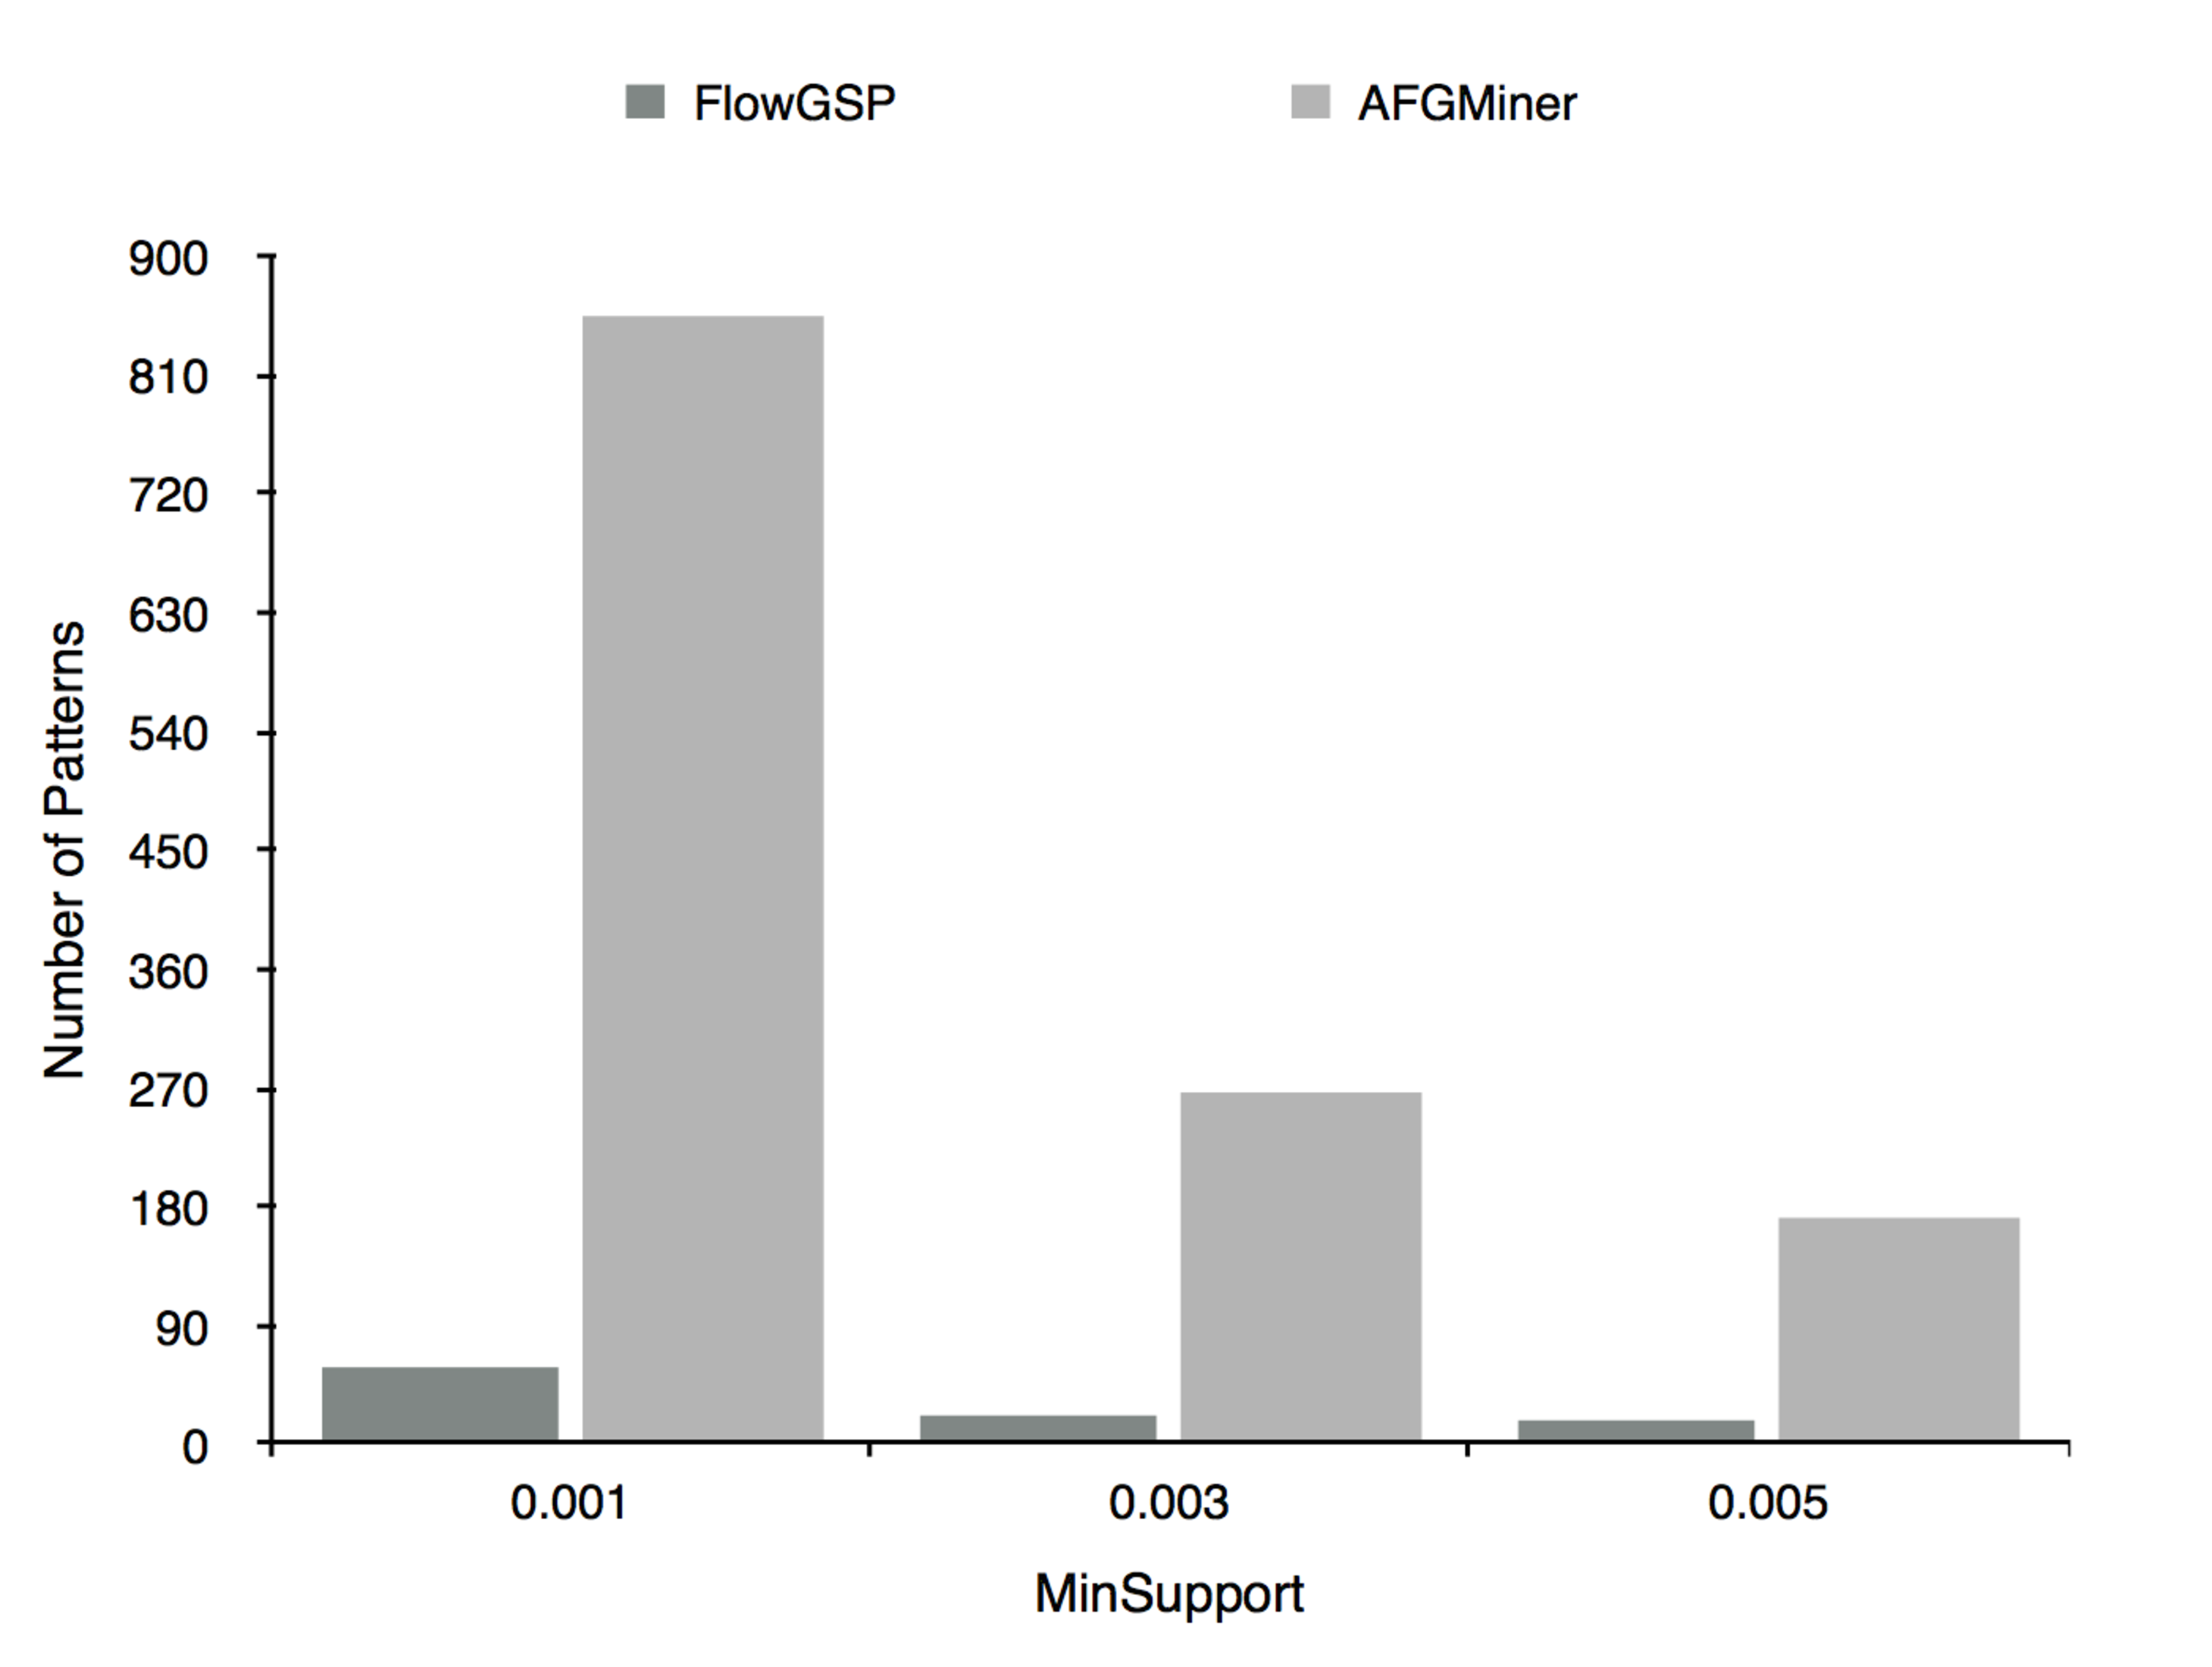
\includegraphics[scale=0.18]{figures/numPatternsComp.pdf}
    \caption{Patterns found by FlowGSP and AFGMiner}
    \label{fig:NumPatterns}
\end{figure}

\subsection{Scalability Analysis}
\label{subsec:Scalability}
From the results of Experiments {\bf A} (Figure~\ref{fig:Plot2}) and {\bf B} (Figure~\ref{fig:Plot1}) we conclude that the MaxAttrs value is not as relevant a factor in the run-time performance of AFGMiner as the number of EFG nodes visited during the mining process. Figure~\ref{fig:Plot2} shows that, in the DayTrader Benchmark, it is more likely that heavyweight patterns have around 7 attributes per node, because making MaxAttrs higher than 7 does not produce statistically significant differences in run-time. It is worth noting that the effects of MaxAttrs on the performance of AFGMiner is dependent on the program being analyzed. If the program's run-time behavior causes more hardware events to happen, then the influence of MaxAttrs is more visible.

Experiment {\bf B} changes the support value in order to increase the number of EFG nodes that the algorithm must visit. Figure~\ref{fig:Plot1} shows that the run-time of AFGMiner scales well enough with the number of EFG nodes visited. The performance of HEPMiner was deemed sufficient for it to be adopted as a handy tool by compiler developers in difficult analysis cases such as applications with flat profiles. However, better candidate pruning techniques could be developed to make AFGMiner faster. If more application-specific versions of the algorithm are developed in the future, those could take into account knowledge about which attributes are more likely to appear in the heavyweight patterns leading to more effective pruning of candidates.

Experiments {\bf C} (Figure~\ref{fig:Plot3}) and {\bf D} (Figure~\ref{fig:Plot4}) show run-times for AFGMiner-locreg and p-AFGMiner, with the number of threads used in parenthesis. As expected, mining becomes faster with more threads being used. However, using more threads has a diminishing effect on run-time decrease as the MinSup or MMH increase. The reason is that, with fewer patterns to mine due to the increase in MinSup/MMH, time spent on data loading and temporary bookkeeping of patterns and pattern occurrences - both done serially by p-AFGMiner - start dominating the total run-time. 

\begin{figure}[h!]
\centering
    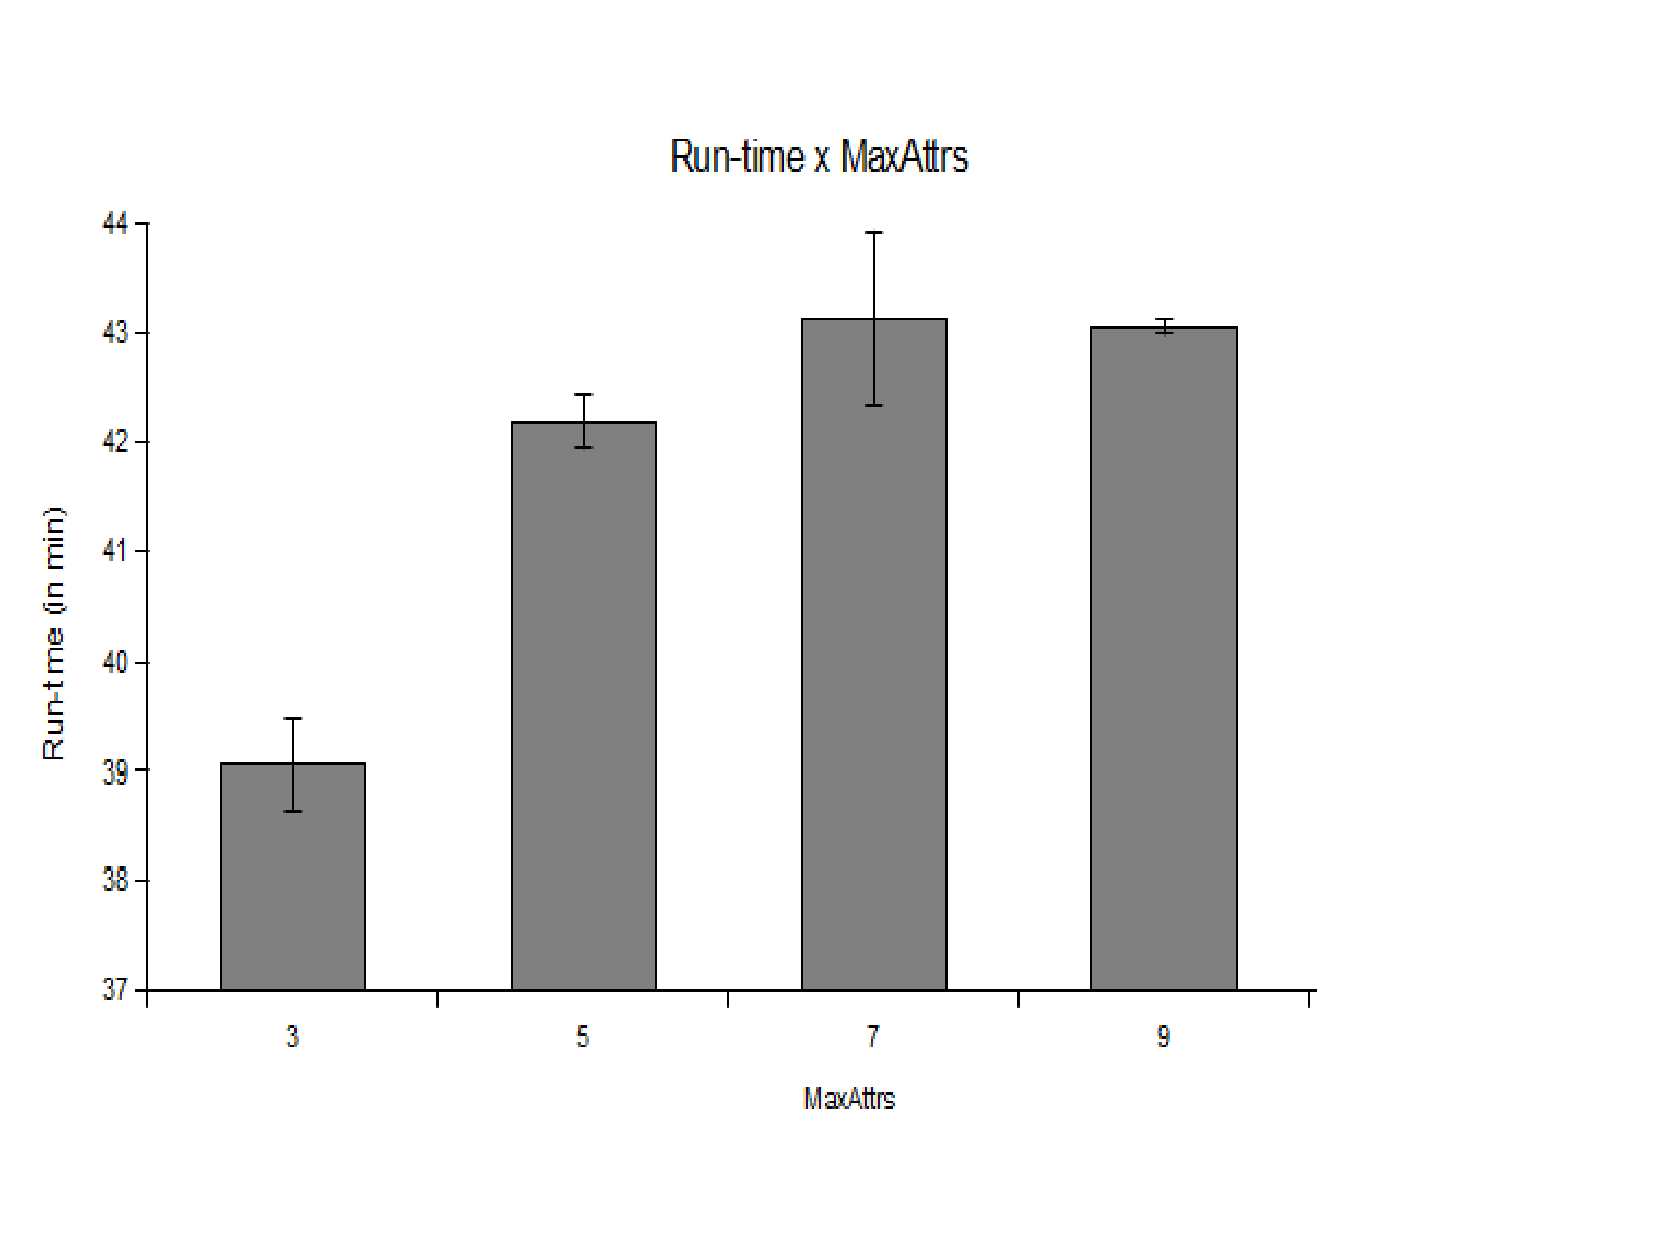
\includegraphics[scale=0.4]{figures/plot2.pdf}
    \caption{Experiment A.}
    \label{fig:Plot2}  
\end{figure}

\begin{figure}[h!]
\centering
    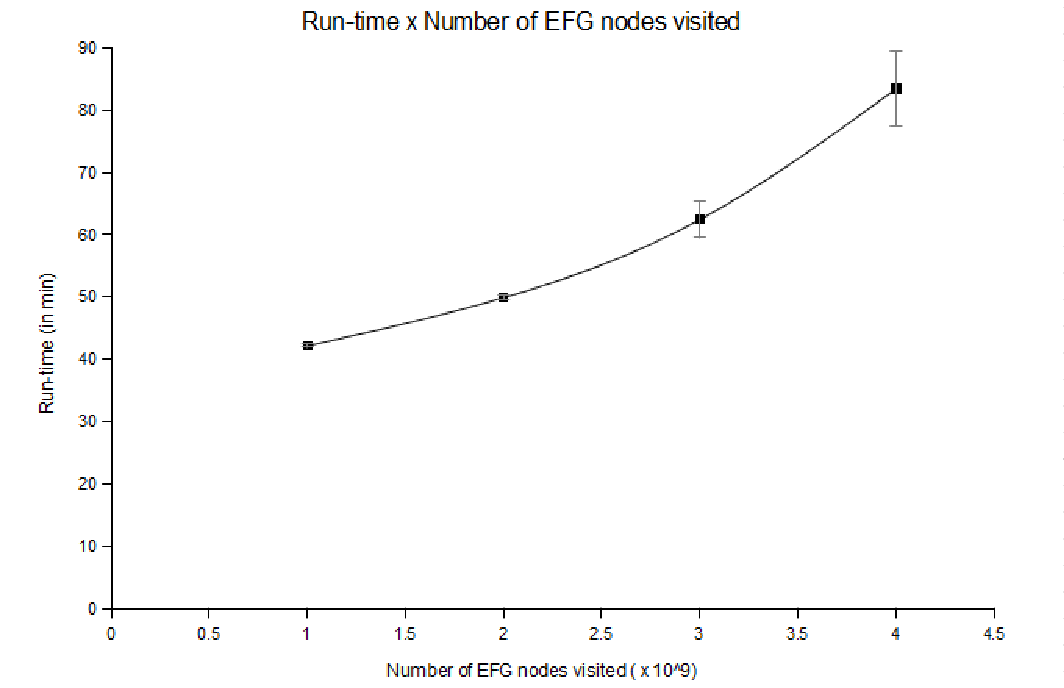
\includegraphics[scale=0.5]{figures/plot1.pdf}
    \caption{Experiment B.}
    \label{fig:Plot1}  
\end{figure}

\begin{figure}[h!]
\centering
    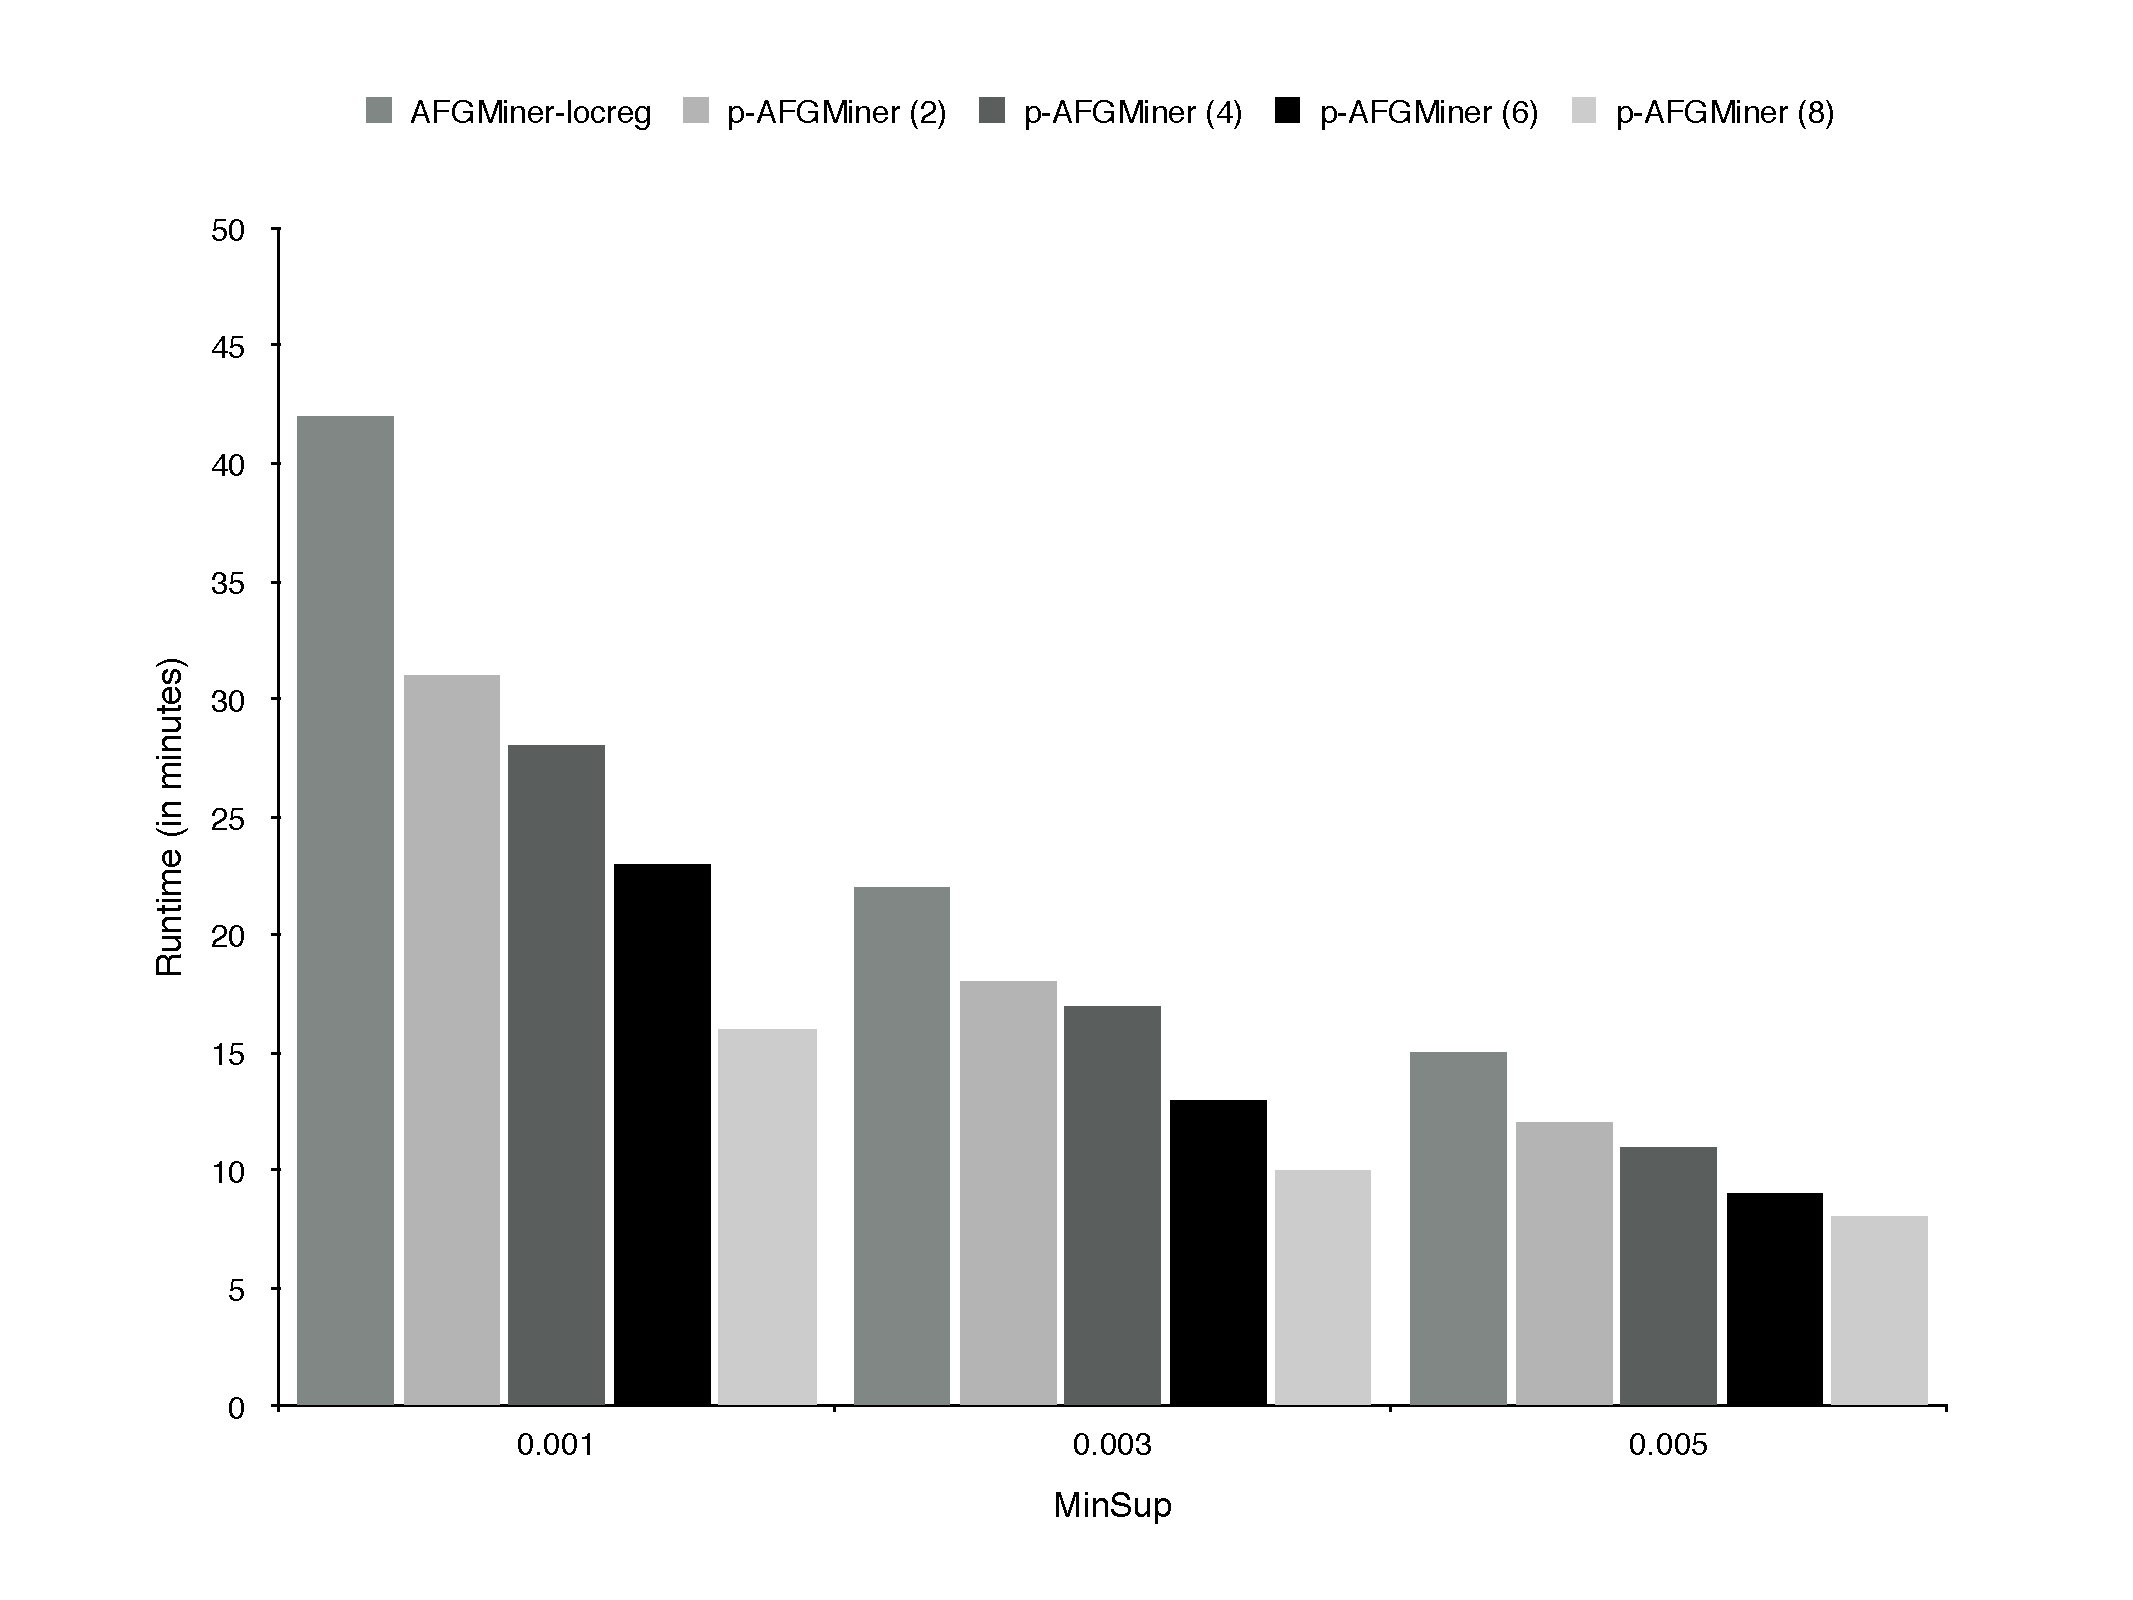
\includegraphics[scale=0.25]{figures/experimentC.pdf}
    \caption{Experiment C.}
    \label{fig:Plot3}  
\end{figure}

\begin{figure}[h!]
\centering
    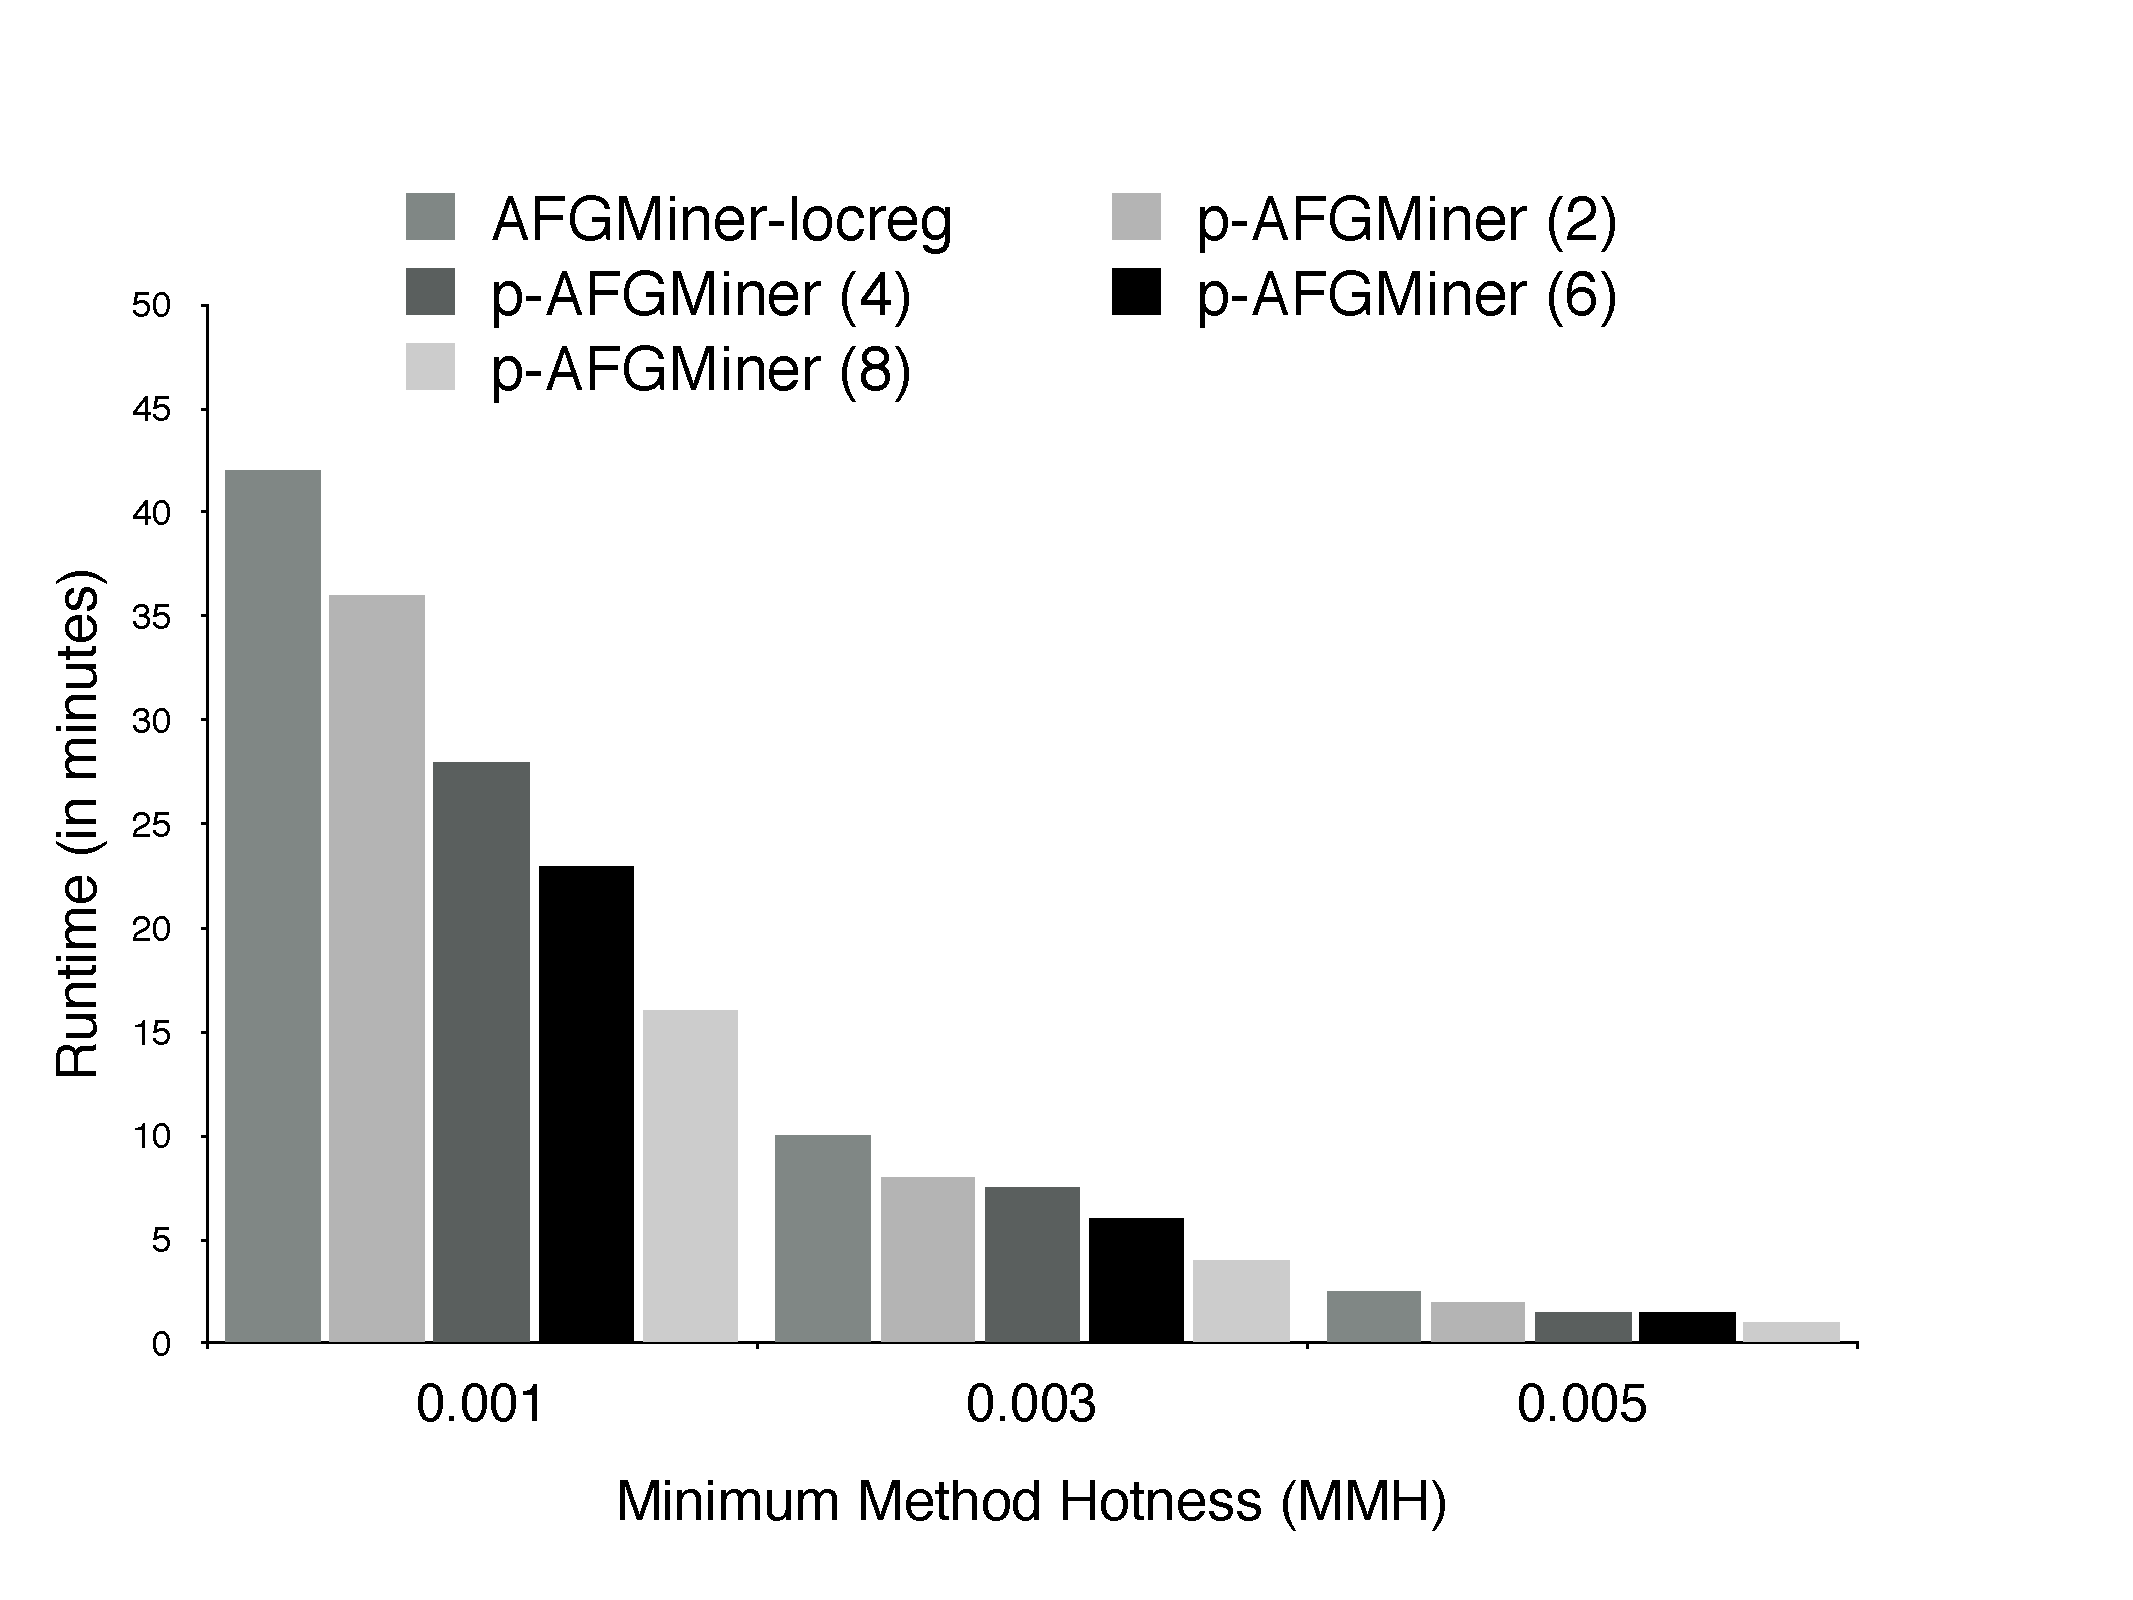
\includegraphics[scale=0.25]{figures/experimentD.pdf}
    \caption{Experiment D.}
    \label{fig:Plot4}  
\end{figure}

\section{Qualitative Analysis}
        \label{sec:QualAnalysis}
        This section discusses the patterns obtained by both HEPMiner. Results were analyzed by compiler engineers from the IBM Canada Software Laboratory. They found HEPMiner to be a useful tool and were able to not only validade results according to previous knowledge about the benchmark, but also to make new observations about the run-time behavior of DayTrader when executed by the z196 hardware. The observations are summarized below.
\begin{enumerate}
\item AFGMiner found heavyweight patterns that contain an edge from a branch instruction leading to a node that has instruction cache misses as one of its attributes. Reviewing the occurrences of such patterns shows that this edge represents the taken path from the branch, which confirms expectation that instruction cache misses should be observed only on the taken branch target.
\item From prior analysis, the experts at IBM know that 30\% of overall CPU cycles in JITted code are assigned to method prologues, and 40\% of instruction cache misses are correlated with method prologues. This was confirmed in the results output by AFGMiner.
\item An attribute that represents a non-taken, correct-direction branch prediction was found to be dominant by AFGMiner. The fact that this attribute shows up highlights that the JIT compiler performs well when ordering basic blocks to optimize for fall-through paths. This discovery led to the creation of performance counters that take into account the ratio of taken and non-taken branches.
\item The relative support values for a sequence of three attributes, present in several patterns, were found to be relevant by the IBM developers. The attributes are an address-generation interlock, followed by a directory or data cache miss, and then an instruction used to load a compressed referenced field from an object. This discovery led to the implementation of the pattern in the compiler's instruction scheduler in order to reduce its negative effect on the run-time of future compiled applications.
\end{enumerate}
\section{Related Work}
	\label{sec:Related}
	FlowGSP is a sequential-pattern mining algorithm that finds patterns whose occurrences are sub-paths of AFGs~\cite{JockschCC10, FlowGSP}. AFGMiner differs from FlowGSP in that it is able to find not only sequential patterns, but also patterns whose occurrences are sub-graphs of AFGs. AFGMiner takes less time than FlowGSP to find each pattern. In addition, AFGMiner is able to map each pattern to all its occurrences and output this mapping to the user.

gSpan is a classic sub-graph mining algorithm. The main difference between AFGMiner and gSpan is that AFGMiner is able to handle multiple node attributes and uses breadth-first search with eager pruning when generating candidate patterns, while gSpan follows a depth-first approach~\cite{gSpan}. \emph{Fast Frequent Subgraph Mining} (FFSM) is another well-known sub-graph mining algorithm for undirected graphs, and its novelty was the introduction of embeddings that make the mining process faster. AFGMiner-locreg also uses embeddings, but has to record the complete mapping between sub-graph patterns and occurrences, making them more memory-consuming. Gaston is a more recent frequent path, tree and graph miner integrated into a single algorithm. In contrast to AFGMiner, however, Gaston only mines for patterns in non-attributed, undirected and unweighted graphs~\cite{Gaston}. \emph{Horvart \etal} describes a sub-graph mining algorithm for outerplanar graphs~\cite{HorvathKDD06}. Similarly to AFGMiner the algorithm runs in incremental polynomial time due to outerplanar graphs being similar enough to trees.

A work related to HEPMiner is that of \emph{Dreweke \etal}. It uses sub-graph mining as part of a code transformation to extract code segments~\cite{DrewekeCGO07}. HEPMiner differs from this work in that it is an external performance analysis tool that helps compiler developers to reach conclusions about the performance of applications of interest, and detect improvement opportunities. 

\section{Future Work}
	\label{sec:Future}
	SCPMiner is another application of AFGMiner and currently a work in progress. It uses AFGMiner to perform profile-based program analysis at the source-code level, finding patterns composed of lines of source-code that, in aggregation, contribute significantly to the total execution time of analyzed flat-profile applications.

In addition, applications of AFGMiner in different domains, such as logistics and social networking, could be developed. The algorithm could also be tuned to take domain-specific knowledge into consideration when searching for candidate patterns and evaluating whether a candidate pattern is heavyweight.

\section*{Conclusion}
	\label{sec:Conclusion}
	This work defined heavyweight patterns and the problem of Heavyweight Pattern Mining. It presented AFGMiner, a heavyweight pattern mining algorithm that is generic enough to be applied to any problem that requires mining of attributed flow graphs, and is able
to find both sub-path and sub-graph patterns. AFGMiner was improved from its original version to use the concepts of location registration. In addition, a parallel version of AFGMiner with location registration was developed that uses a workload distribution heuristic to better balance the mining work performed by different threads.

The tools HEPMiner and SCPMiner, targeted at compiler and application developers, respectively, were created as useful applications of AFGMiner. The heavyweight patterns obtained by such tools were positively evaluated by experts from the IBM Canada Software Laboratory and gave them useful insight into the run-time behavior of analyzed programs.



%\section{Introduction}
% no \IEEEPARstart
%This demo file is intended to serve as a ``starter file''
%for IEEE conference papers produced under \LaTeX\ using
%IEEEtran.cls version 1.7 and later.
% You must have at least 2 lines in the paragraph with the drop letter
% (should never be an issue)
%I wish you the best of success.

%\hfill mds
 
%\hfill January 11, 2007

%\subsection{Subsection Heading Here}
%Subsection text here.


%\subsubsection{Subsubsection Heading Here}
%Subsubsection text here.


% An example of a floating figure using the graphicx package.
% Note that \label must occur AFTER (or within) \caption.
% For figures, \caption should occur after the \includegraphics.
% Note that IEEEtran v1.7 and later has special internal code that
% is designed to preserve the operation of \label within \caption
% even when the captionsoff option is in effect. However, because
% of issues like this, it may be the safest practice to put all your
% \label just after \caption rather than within \caption{}.
%
% Reminder: the "draftcls" or "draftclsnofoot", not "draft", class
% option should be used if it is desired that the figures are to be
% displayed while in draft mode.
%
%\begin{figure}[!t]
%\centering
%\includegraphics[width=2.5in]{myfigure}
% where an .eps filename suffix will be assumed under latex, 
% and a .pdf suffix will be assumed for pdflatex; or what has been declared
% via \DeclareGraphicsExtensions.
%\caption{Simulation Results}
%\label{fig_sim}
%\end{figure}

% Note that IEEE typically puts floats only at the top, even when this
% results in a large percentage of a column being occupied by floats.


% An example of a double column floating figure using two subfigures.
% (The subfig.sty package must be loaded for this to work.)
% The subfigure \label commands are set within each subfloat command, the
% \label for the overall figure must come after \caption.
% \hfil must be used as a separator to get equal spacing.
% The subfigure.sty package works much the same way, except \subfigure is
% used instead of \subfloat.
%
%\begin{figure*}[!t]
%\centerline{\subfloat[Case I]\includegraphics[width=2.5in]{subfigcase1}%
%\label{fig_first_case}}
%\hfil
%\subfloat[Case II]{\includegraphics[width=2.5in]{subfigcase2}%
%\label{fig_second_case}}}
%\caption{Simulation results}
%\label{fig_sim}
%\end{figure*}
%
% Note that often IEEE papers with subfigures do not employ subfigure
% captions (using the optional argument to \subfloat), but instead will
% reference/describe all of them (a), (b), etc., within the main caption.


% An example of a floating table. Note that, for IEEE style tables, the 
% \caption command should come BEFORE the table. Table text will default to
% \footnotesize as IEEE normally uses this smaller font for tables.
% The \label must come after \caption as always.
%
%\begin{table}[!t]
%% increase table row spacing, adjust to taste
%\renewcommand{\arraystretch}{1.3}
% if using array.sty, it might be a good idea to tweak the value of
% \extrarowheight as needed to properly center the text within the cells
%\caption{An Example of a Table}
%\label{table_example}
%\centering
%% Some packages, such as MDW tools, offer better commands for making tables
%% than the plain LaTeX2e tabular which is used here.
%\begin{tabular}{|c||c|}
%\hline
%One & Two\\
%\hline
%Three & Four\\
%\hline
%\end{tabular}
%\end{table}


% Note that IEEE does not put floats in the very first column - or typically
% anywhere on the first page for that matter. Also, in-text middle ("here")
% positioning is not used. Most IEEE journals/conferences use top floats
% exclusively. Note that, LaTeX2e, unlike IEEE journals/conferences, places
% footnotes above bottom floats. This can be corrected via the \fnbelowfloat
% command of the stfloats package.

% conference papers do not normally have an appendix


% use section* for acknowledgement
\section*{Acknowledgments}
This research is partially funded by a grant from the Natural Science and Engineering Research Council of Canada through a Collaborative Research and Development grant and by the IBM Centre for Advanced Studies

% trigger a \newpage just before the given reference
% number - used to balance the columns on the last page
% adjust value as needed - may need to be readjusted if
% the document is modified later
%\IEEEtriggeratref{8}
% The "triggered" command can be changed if desired:
%\IEEEtriggercmd{\enlargethispage{-5in}}

% references section

% can use a bibliography generated by BibTeX as a .bbl file
% BibTeX documentation can be easily obtained at:
% http://www.ctan.org/tex-archive/biblio/bibtex/contrib/doc/
% The IEEEtran BibTeX style support page is at:
% http://www.michaelshell.org/tex/ieeetran/bibtex/
%\bibliographystyle{IEEEtran}
% argument is your BibTeX string definitions and bibliography database(s)
%\bibliography{IEEEabrv,../bib/paper}
%
% <OR> manually copy in the resultant .bbl file
% set second argument of \begin to the number of references
% (used to reserve space for the reference number labels box)
%\begin{thebibliography}{1}

%\bibitem{IEEEhowto:kopka}
%H.~Kopka and P.~W. Daly, \emph{A Guide to \LaTeX}, 3rd~ed.\hskip 1em plus
% 0.5em minus 0.4em\relax Harlow, England: Addison-Wesley, 1999.

%\end{thebibliography}

\bibliographystyle{IEEEtran}
\bibliography{local}  

% that's all folks
\end{document}


